%%%%%%%%%%%%%%%%%%%%%%%%%%%%%%%%%%%%%%%%%%%%%%%%%%%%%%%%%%%%%%%%%
\chapter{RESULTS}
\label{ch:CH6}
%%%%%%%%%%%%%%%%%%%%%%%%%%%%%%%%%%%%%%%%%%%%%%%%%%%%%%%%%%%%%%%%%

\section{Performance Measurement}

\subsection{Confusion Matrix}

The confusion matrix is a table that constructed to visualize the performance of classifier. It includes actual and predicted results for each class on the corresponding task. In our study, the rows specifies the actual results while columns specifies predicted ones.

During the performance measurement, the focused class is called as Positive (P), and the others are as Negatives (N). For binary classification problems, which is as in our study, one class can be directly specified as P and the other as N. We indicated the COVID-19 label as Positive class, and the non-COVID-19 label as Negative class.

If a sample in actual P class is predicted as in P class, then it is a True Positive (TP) sample, otherwise it is False Positive (FP). On the other hand, if a sample in actual N class is predicted as in P class, then it is a False Negative (FN) sample, otherwise it is True Negative (TN).

From the definitions, the following equalities can be easily derived: P = TP + FN and N = FP + TN.

\begin{table*}[!h]
	{
		\setlength{\tabcolsep}{14pt}
		\caption{Sample Confusion Matrix.}
		\begin{center}
			% \vspace{-6mm}
			\begin{tabular}{|c|l|l|l|}
				\hline
				\multicolumn{2}{|c|}{\multirow{2}{*}{\begin{tabular}[c]{@{}c@{}}\\CONFUSION\\ MATRIX\end{tabular}}} & \multicolumn{2}{c|}{Actual} \\ 
				\cline{3-4} 
				\multicolumn{2}{|c|}{}                                                                            & \begin{tabular}[c]{@{}l@{}}\quad\quad P \\ (COVID-19)\end{tabular} & \begin{tabular}[c]{@{}l@{}}\quad\quad N \\ (non-COVID-19)\end{tabular} \\ 
				\hline
				\multirow{2}{*}{Predicted}      & \begin{tabular}[c]{@{}l@{}} \quad\quad P \\ (COVID-19)\end{tabular}         & \textbf{TP}                                             & FN                                                          \\
				\cline{2-4} 
				& \begin{tabular}[c]{@{}l@{}} \quad\quad N \\ (non-COVID-19)\end{tabular}     & FP                                                      & \textbf{TN}                                                 \\ \hline
			\end{tabular}
			% \vspace{-6mm}
		\end{center}
		\label{sample_confusion_matrix}
	}
\end{table*}

\subsection{The Analysis of Confusion Matrix}

Various meaningful ratios can be extracted from the confusion matrix. In this section, we study the significant ones which were also used in the thesis to measure the performance on our tasks.

We computed the metrics Sensitivity, Specificity, Precision, Accuracy and F1-Score in a weighted way. That is, these stated metrics were computed for each class and then taken the weighted average as in:

\be
\label{eq:weighted_avg_metric}
\frac{\sum_{i=1}^{m} (\text{the metric value for class i}) \times (\text{the number of test samples in class i})} {(\text{the total number of test samples})} \:\: \raisepunct{.}
\ee

Recall that the task we worked on is a binary classification problem. That is, $m$ was 2 in our computations. So that, the average value for metric $M$ of an experiment, where M is one of Sensitivity, Specificity, Precision, Accuracy and F1-Score metrics, was computed as:

\be
\label{eq:weighted_avg_binary_class_metric}
M = \frac{M_{c_{1}} \times n_{c_{1}} + M_{c_{2}} \times n_{c_{2}}} {n_{c_{1}} + n_{c_{2}}} \:\: \raisepunct{,}
\ee

where $M_{c_{1}},\:\:M_{c_{2}},\:\:n_{c_{1}}\:\:\text{and}\:\:n_{c_{2}}$ refer the value of $M$ for class 1, the value of $M$ for class 2, the number of test samples in class 1 and the number of test samples in class 2 respectively.

\subsubsection{Sensitivity (True Positive Rate - TPR)}

Sensitivity (TPR) measures the ratio of positive class samples predicted correctly over all samples predicted as positive as given below:

\begin{equation}
	\label{eq:TPR}
	TPR = \frac{TP}{P} = \frac{TP}{TP + FN}\raisepunct{.}
\end{equation}

\subsubsection{Specificity (True Negative Rate - TNR)}

Specificity (TNR) measures the ratio of negative class samples predicted correctly over all samples predicted as negative as given below:

\begin{equation}
	\label{eq:TNR}
	TNR = \frac{TN}{N} = \frac{TN}{FP + TN}\raisepunct{.}
\end{equation}

\subsubsection{Precision (Positive Predictive Value - PPV)}

Precision (PPV) measures the ratio of correctly predicted positive class samples over all samples having actual positive label as given below:

\begin{equation}
	\label{eq:PPV}
	PPV = \frac{TP}{TP + FP}\raisepunct{.}
\end{equation}

\subsubsection{Accuracy (ACC)}

Accuracy (ACC) measures the ratio of correctly predicted samples over all samples as given below:

\begin{equation}
	\label{eq:ACC}
	ACC = \frac{TP + TN}{P + N} = \frac{TP + TN}{TP + FP + FN + TN}\raisepunct{.}
\end{equation}

\subsubsection{F1 Score}

F1 Score is the harmonic mean of sensitivity and precision as given below:

\begin{equation}
	\label{eq:F1_Score}
	F_{1} = 2 \times \frac{PPV \times TPR}{PPV + TPR} = \frac{2 \times TP}{2 \times TP + FP + FN}\raisepunct{.}
\end{equation}

\subsubsection{Area Under the Curve (AUC Score)}

Area Under the Curve (AUC Score) measures the probability of classifier to rank a randomly chosen positive sample higher than a random chosen negative sample (under the assumption that "positive" ranks are higher than "negative" ranks) for normalized samples. The computation of AUC Score value is as given below:

\begin{align}
	\label{eq:AUC_Score}
	\nonumber
	& TPR(t) : t \rightarrow y \left ( x \right ), \\
	\nonumber
	& FPR(t) : t \rightarrow x, \:\: \text{and} \\ 
	& AUC = \int_{0}^{1} TPR \left ( FPR^{-1}\left ( x \right ) \right ) dx = \int_{-\infty}^{\infty} TPR \left ( t \right ) \times {FPR}' \left ( t \right ) dt.
\end{align}

\section{Convolutional Neural Network Results}

Here, we report the results of convolutional neural network experiments explained in Section~\ref{sec:CH5_cnn_experiments}. As stated, AlexNet, ResNet-18, ResNet-34, ResNet-50, VGG-16 and VGG-19 architectures were trained initialized by their pre-trained weights with three different optimizers such that SGD with momentum, Adam and Adam with decoupled weight decay. The accuracy and loss curves for three different optimizers on train and validation processes can be viewed on Figures~\ref{fig:alexnet_plots} - \ref{fig:vgg19_plots} whose x-axis represent the number of epochs. The plots were created by TensorBoard platform prepared with the Python TensorFlow package version 2.3.1. Additional required package versions are as follows: 1) TensorFlow Addons with the version of 0.11.2, 2) TensorFlow Estimator with the version of 2.3.0, 3) TensorFlow Hub with the version of 0.10.0, and 4) TensorFlow Probability with the version of 0.10.0.

The results can be also seen in Table~\ref{tab:cnn_result_table} including accuracy, sensitivity, specificity, precision and F1 score values, and loss values for last train epoch and test run. We obtained the best result from ResNet-50 model after $9^{th}$ train epoch in 7 minutes with the accuracy, sensitivity, specificity, precision, F1 score and AUC score of 92.16\%, 0.9216, 0.9215, 0.9216, 0.9216, 0.9215 respectively, and the loss of $9^{th}$ train epoch and validation as 0.0223 and 1.3687.

\begin{figure}[!h]
	\centering
	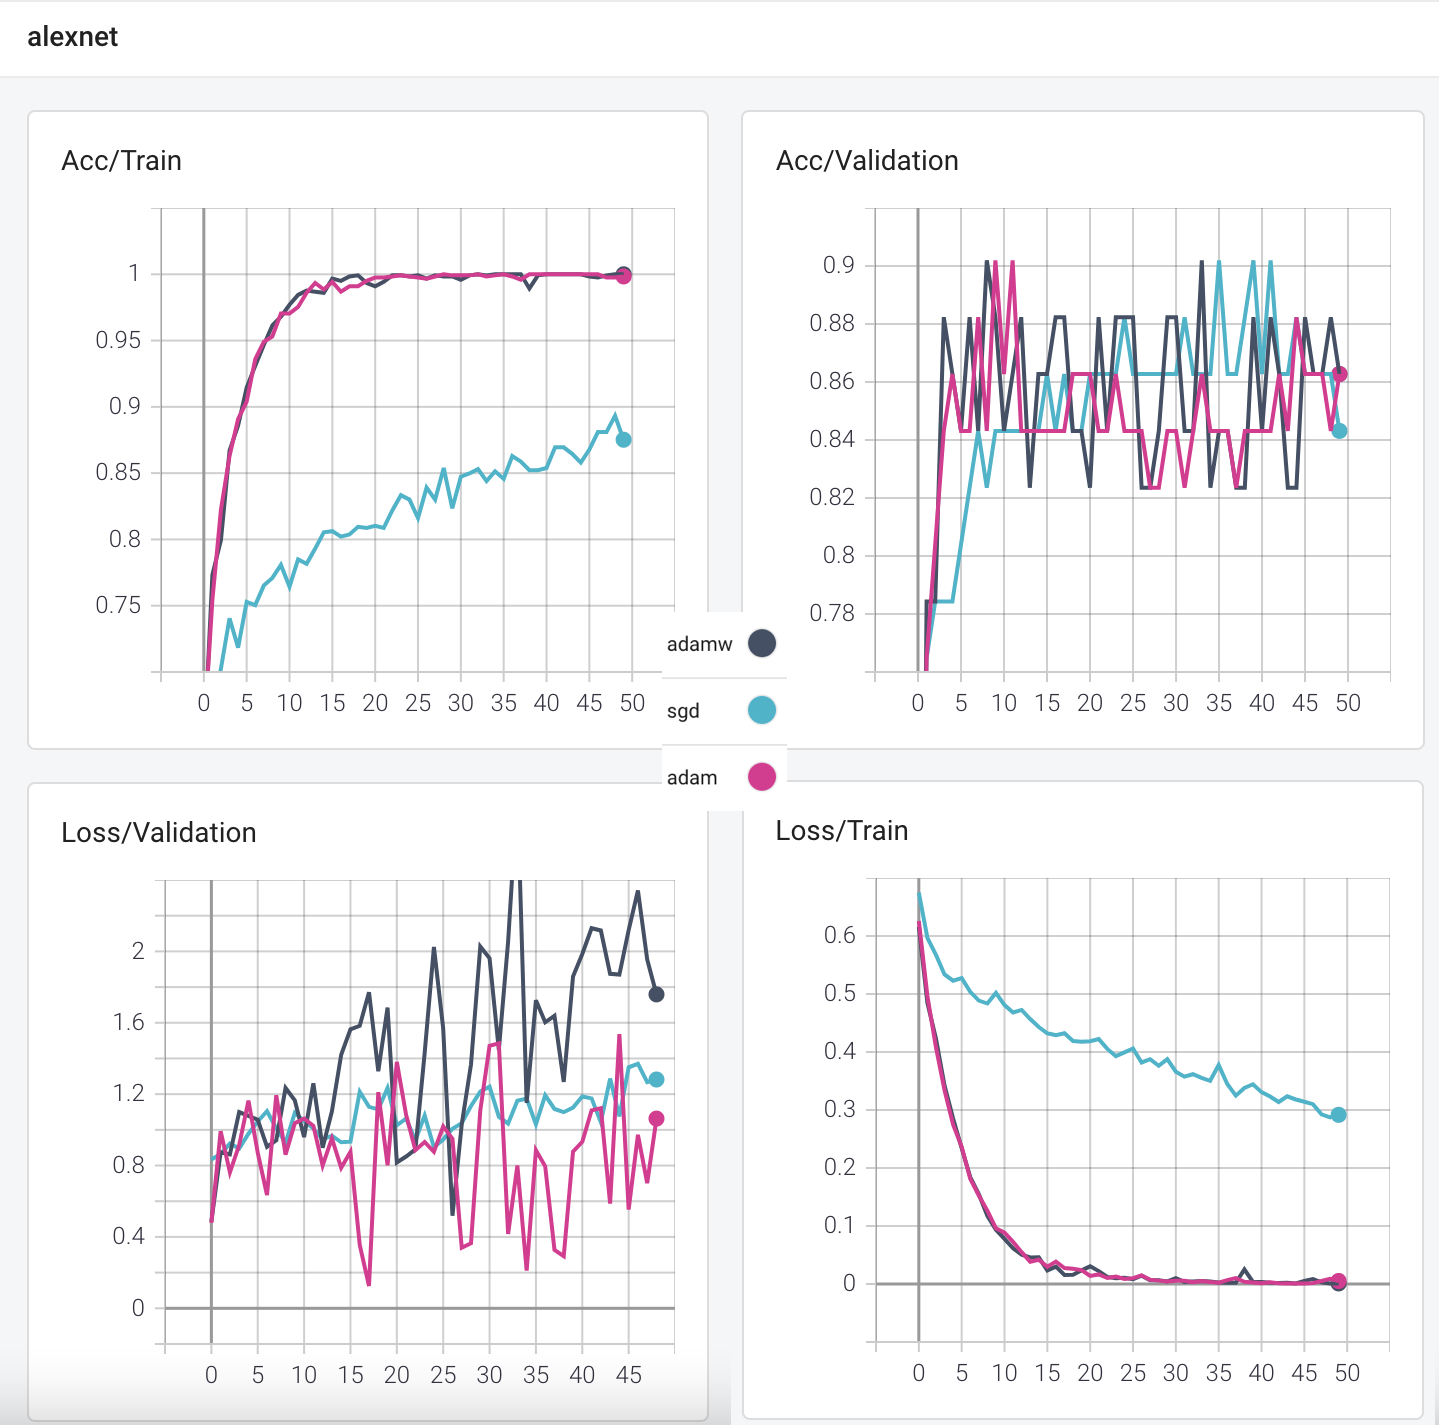
\includegraphics[width=\linewidth]{fig/alexnet.png}
	\vspace{2mm}
	\caption{AlexNet model accuracy and loss curves for three different optimizers on train and validation processes.}
	\label{fig:alexnet_plots}
\end{figure}

\begin{figure}[!h]
	\centering
	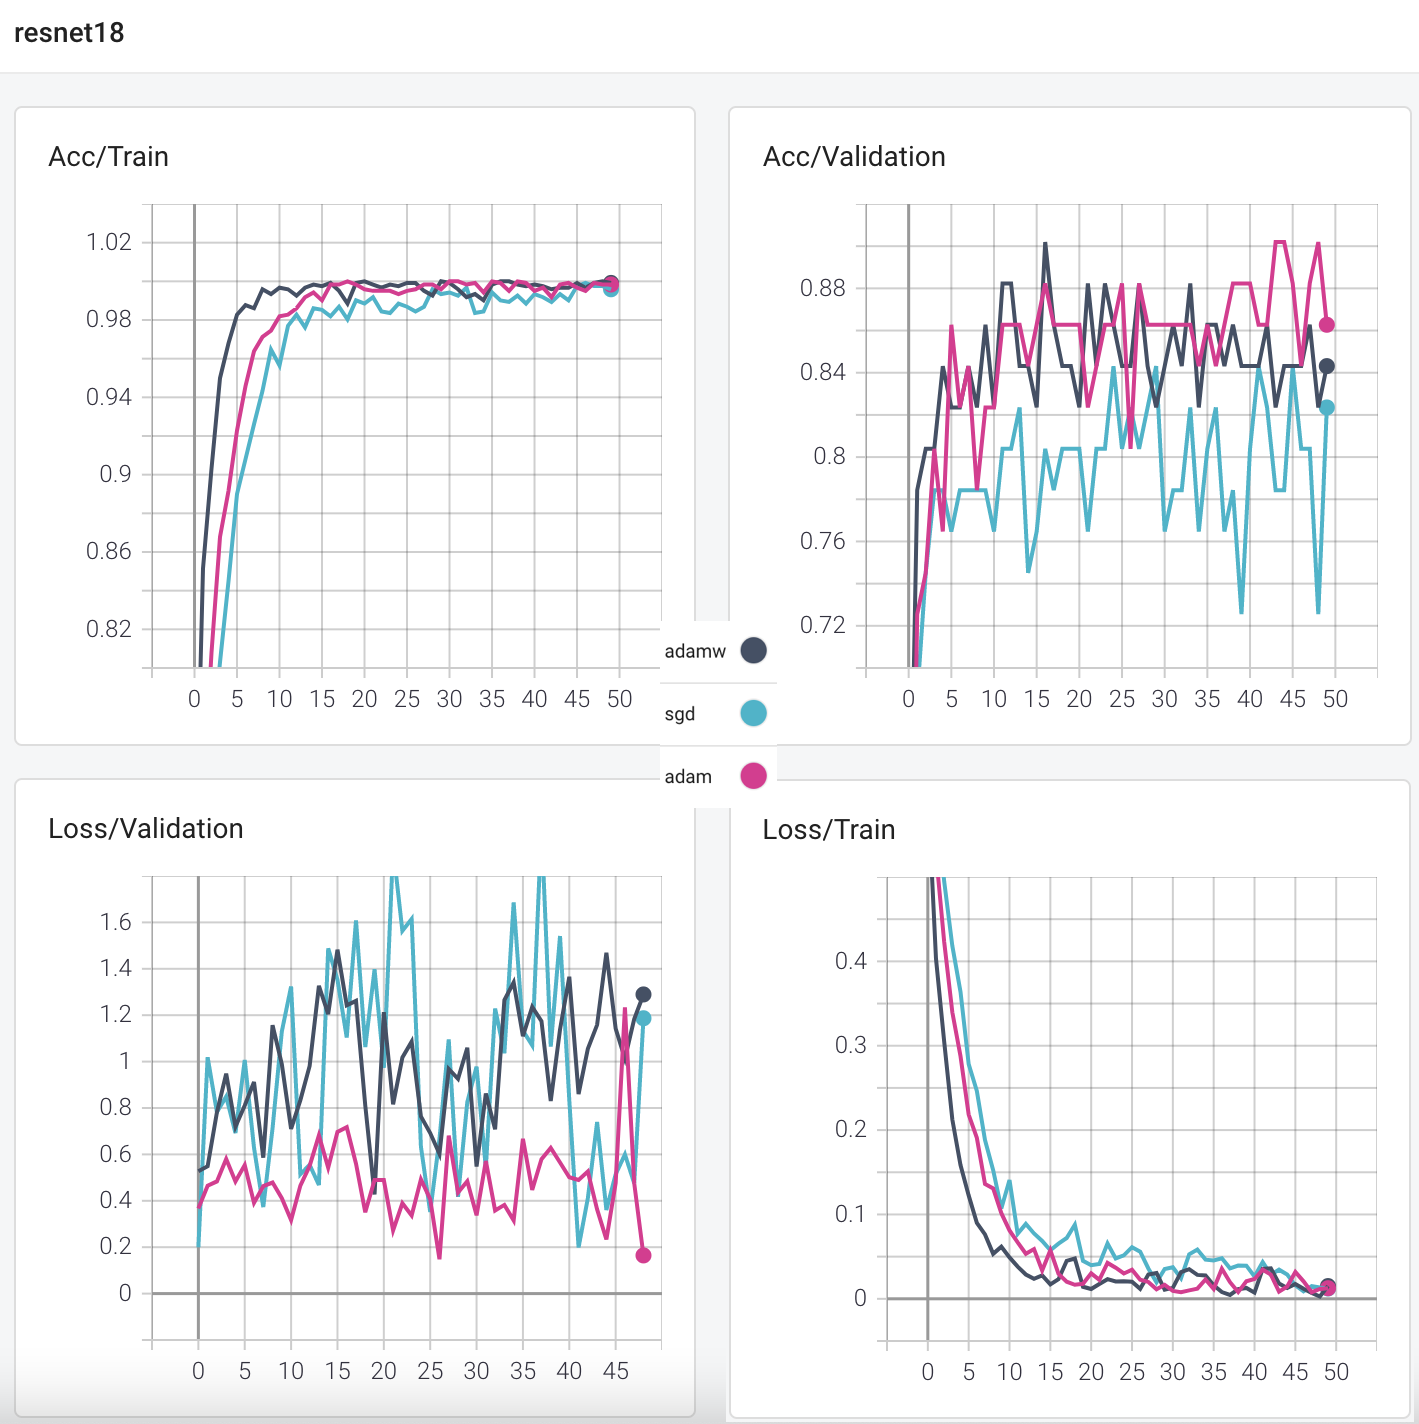
\includegraphics[width=\linewidth]{fig/resnet18.png}
	\vspace{2mm}
	\caption{ResNet-18 model accuracy and loss curves for three different optimizers on train and validation processes.}
	\label{fig:resnet18_plots}
\end{figure}

\begin{figure}[!h]
	\centering
	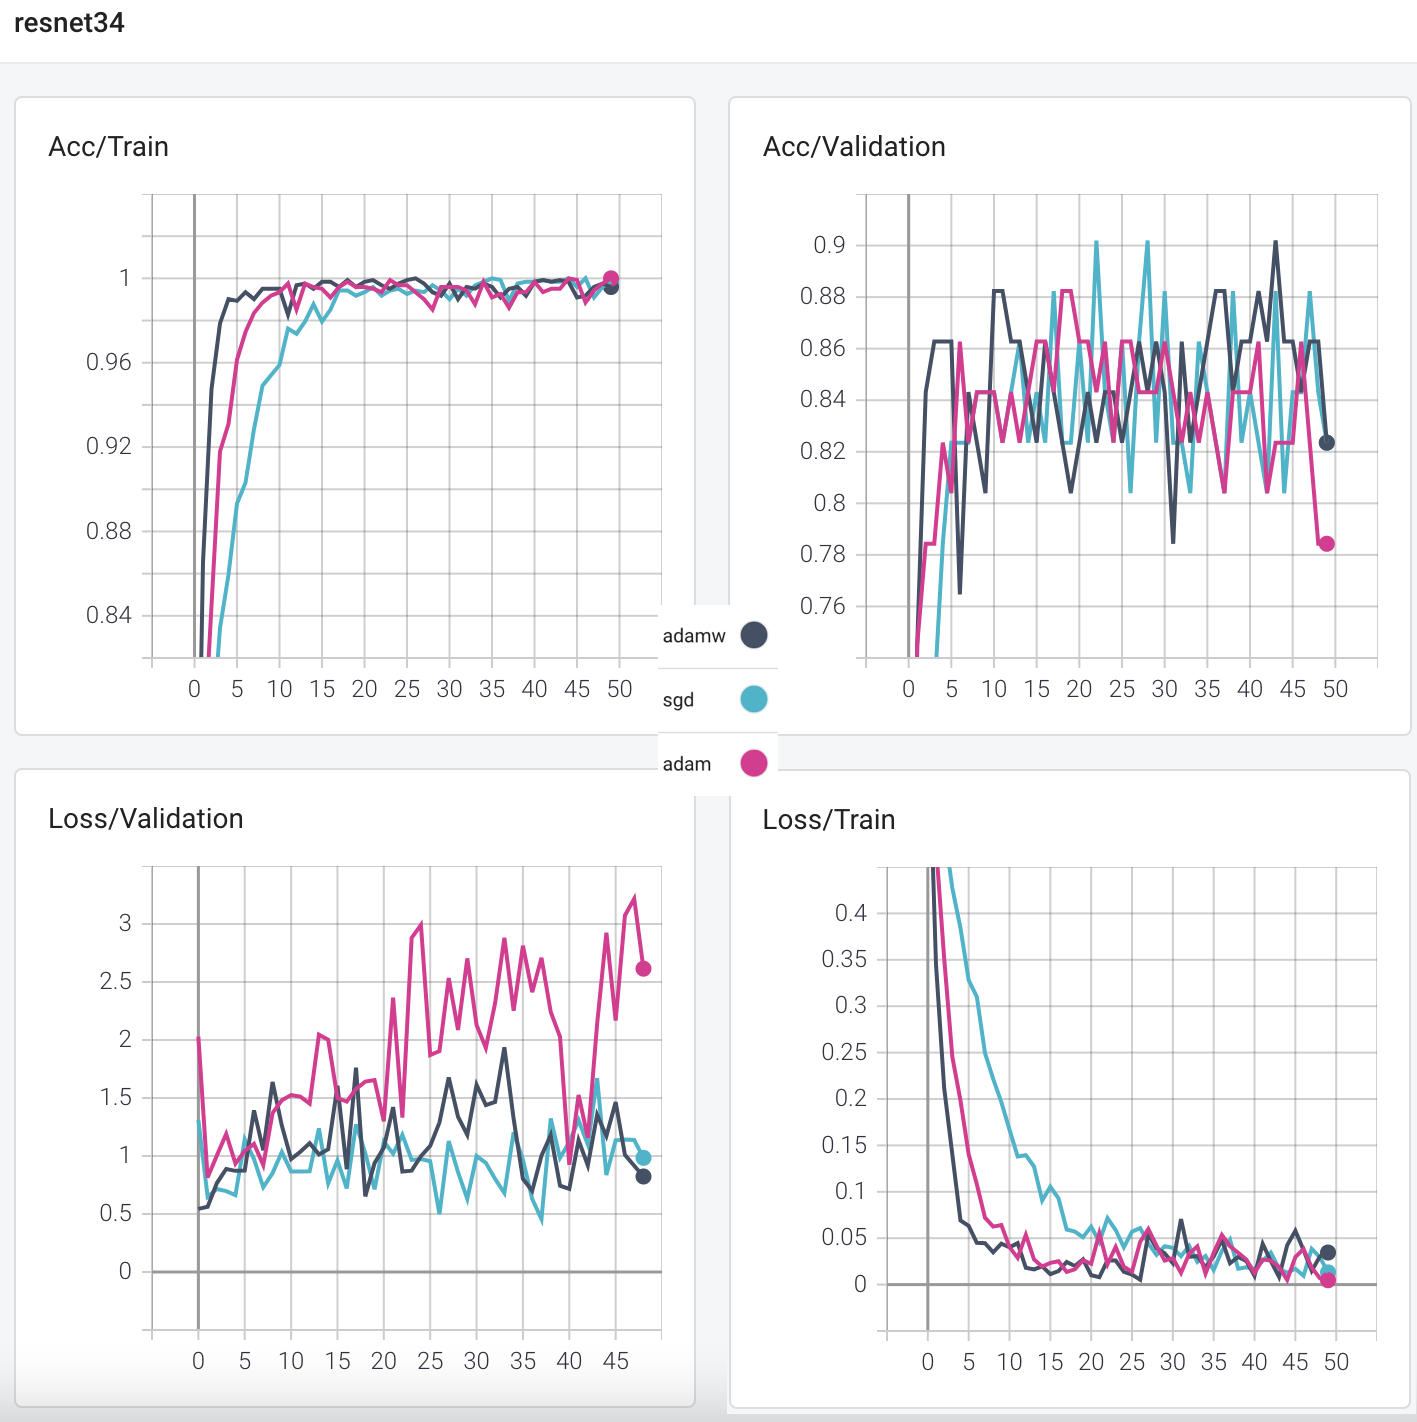
\includegraphics[width=\linewidth]{fig/resnet34.png}
	\vspace{2mm}
	\caption{ResNet-34 model accuracy and loss curves for three different optimizers on train and validation processes.}
	\label{fig:resnet34_plots}
\end{figure}

\begin{figure}[!h]
	\centering
	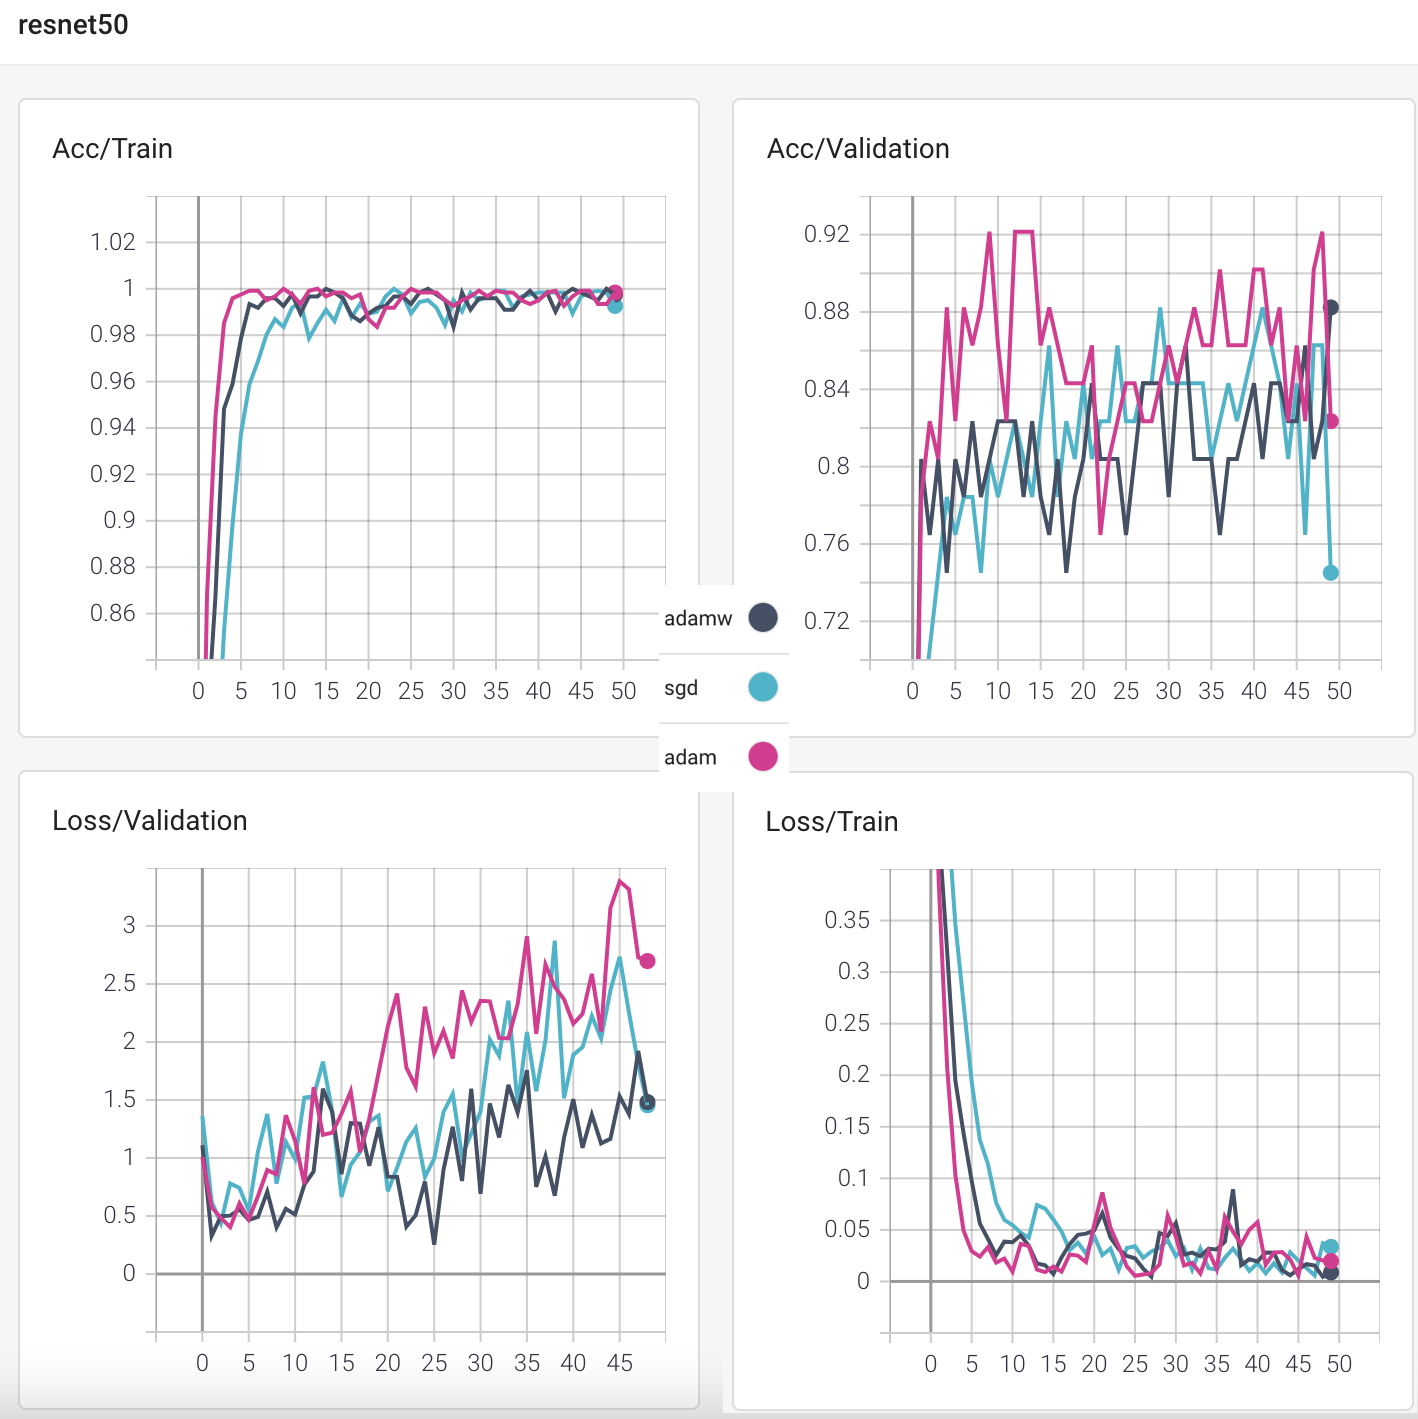
\includegraphics[width=\linewidth]{fig/resnet50.png}
	\vspace{2mm}
	\caption{ResNet-50 model accuracy and loss curves for three different optimizers on train and validation processes.}
	\label{fig:resnet50_plots}
\end{figure}

\begin{figure}[!h]
	\centering
	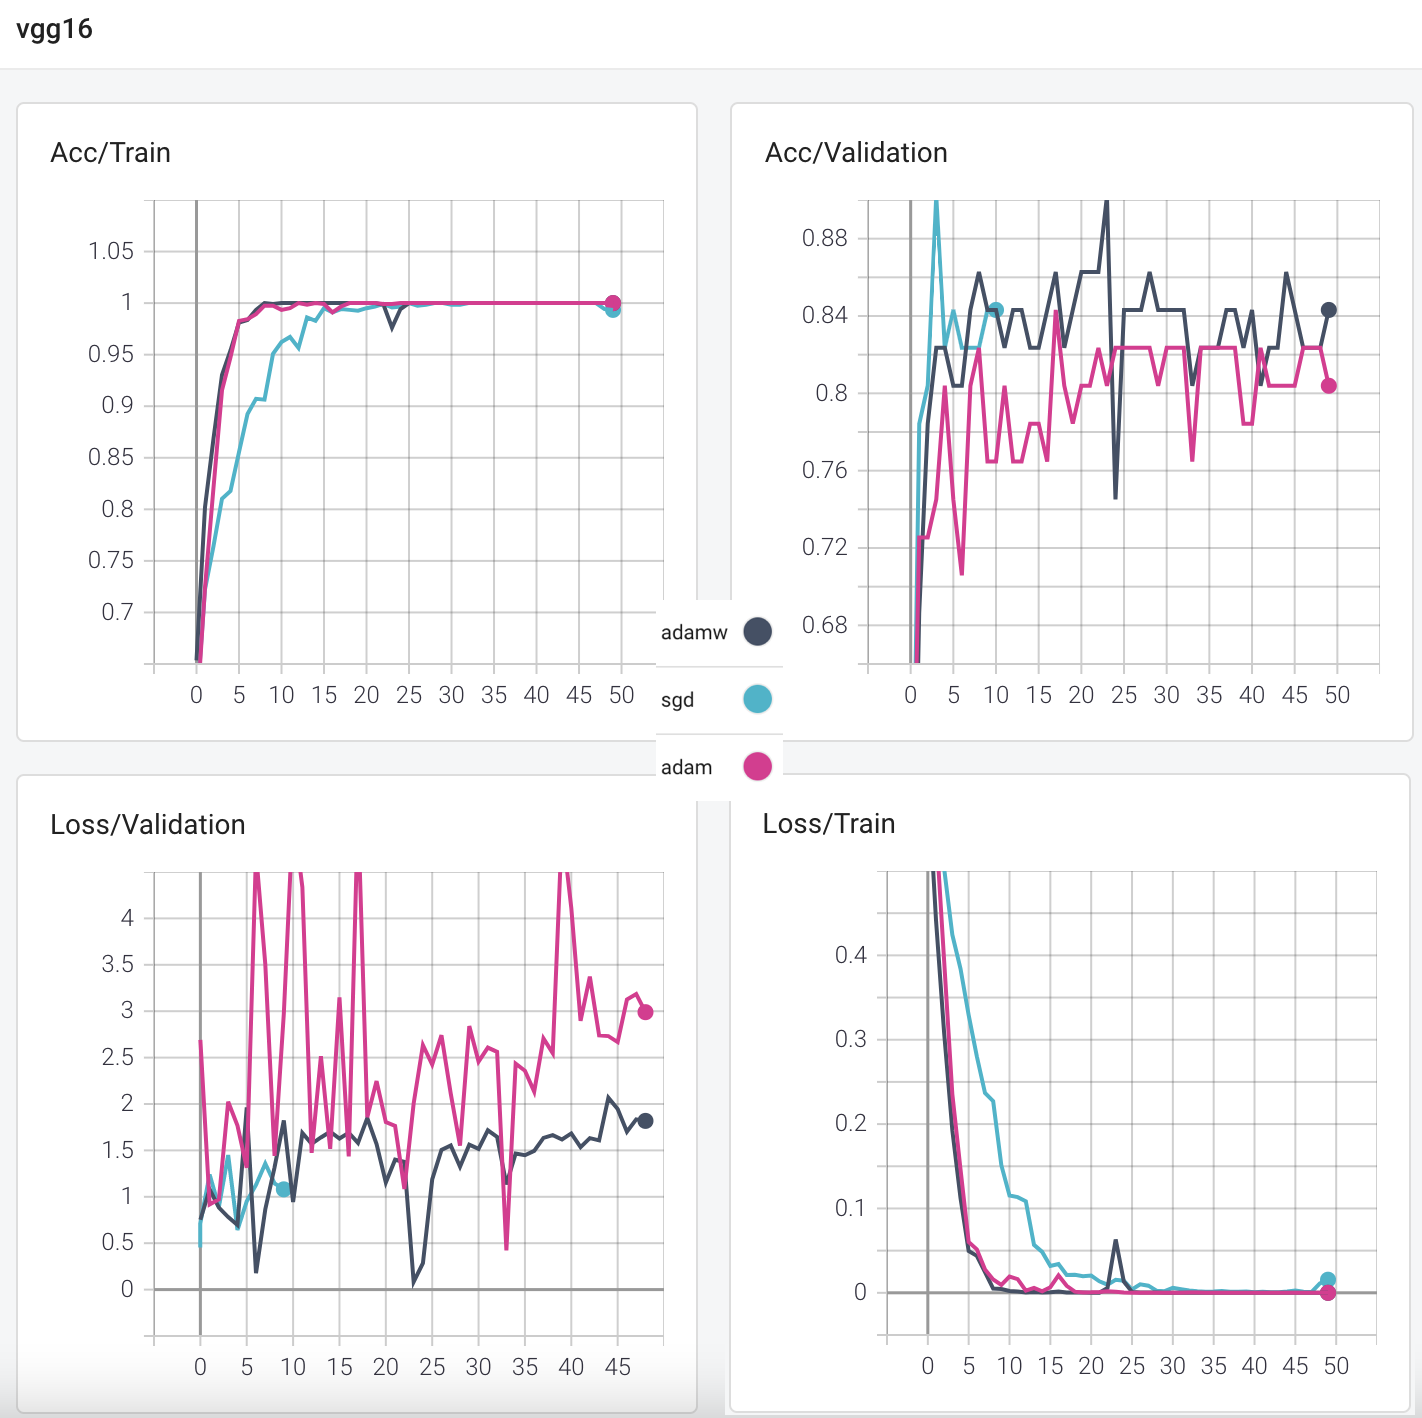
\includegraphics[width=\linewidth]{fig/vgg16.png}
	\vspace{2mm}
	\caption{VGG16 model accuracy and loss curves for three different optimizers on train and validation processes.}
	\label{fig:vgg16_plots}
\end{figure}

\begin{figure}[!h]
	\centering
	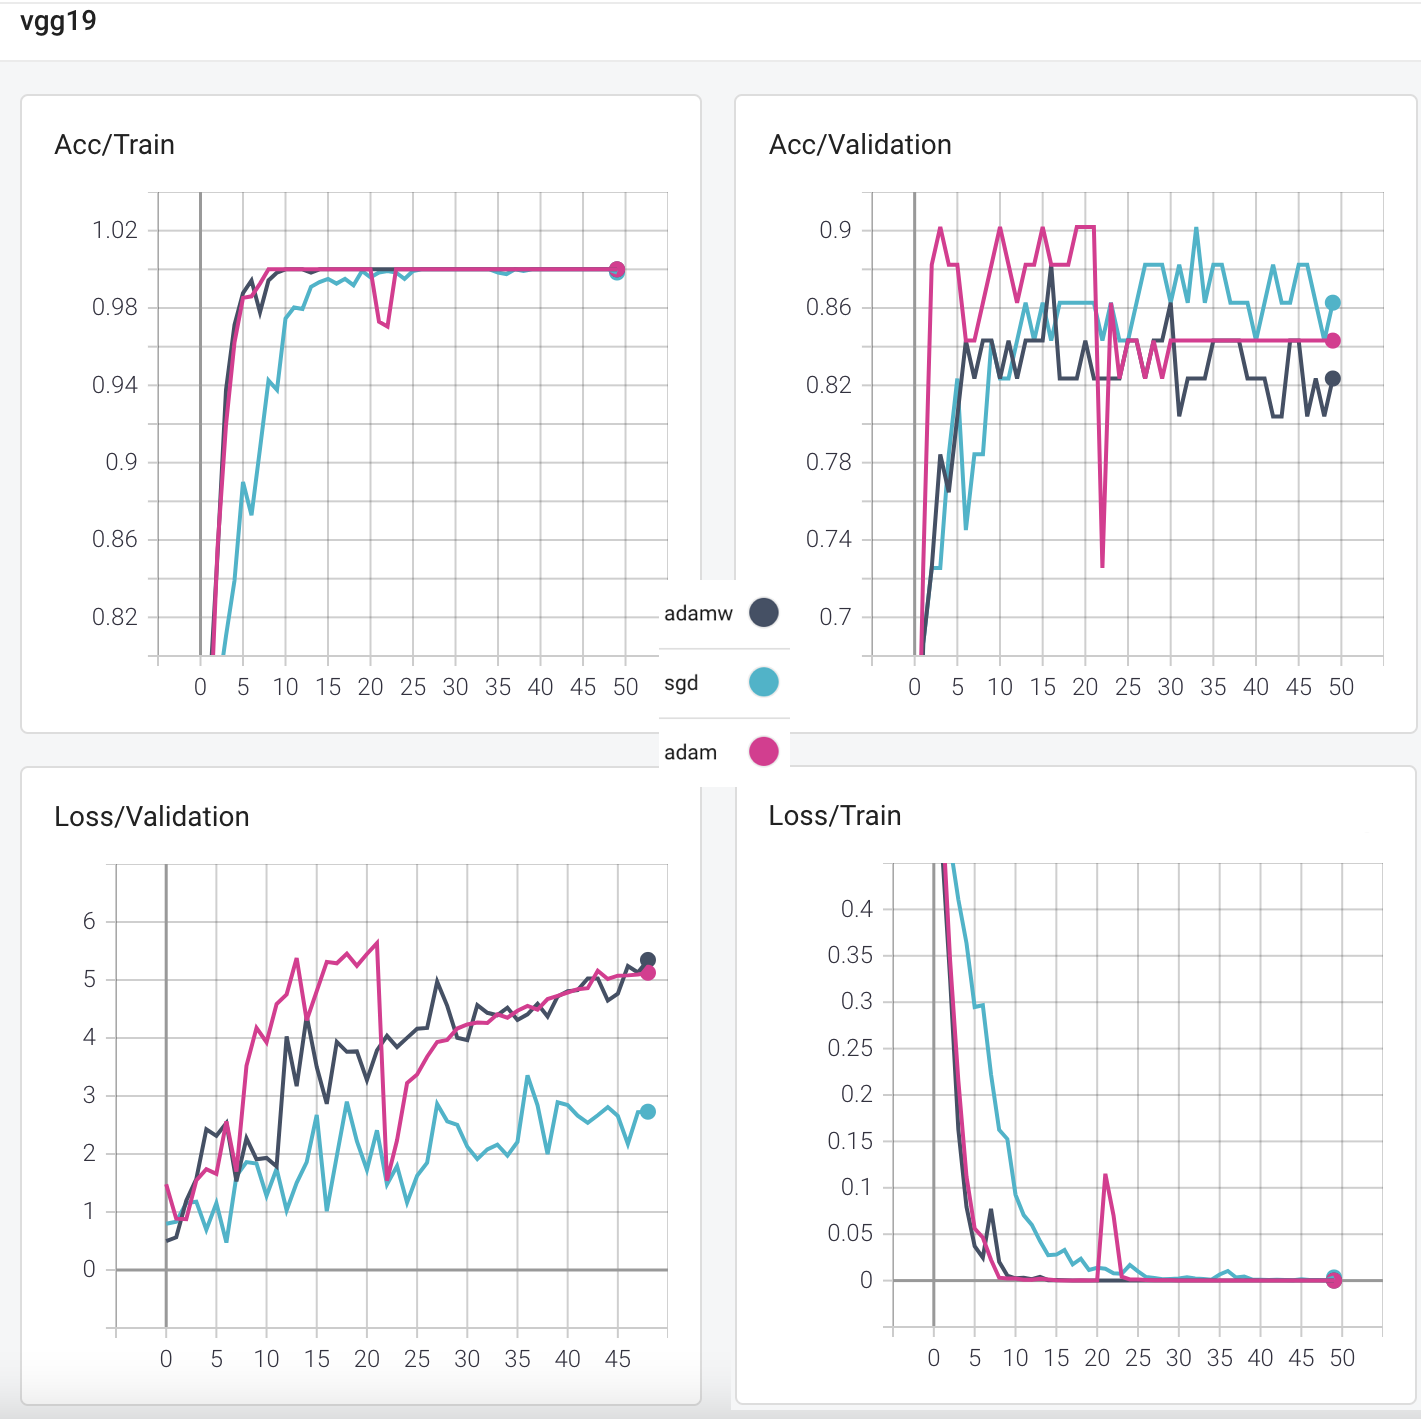
\includegraphics[width=\linewidth]{fig/vgg19.png}
	\vspace{2mm}
	\caption{VGG19 model accuracy and loss curves for three different optimizers on train and validation processes.}
	\label{fig:vgg19_plots}
\end{figure}

% Please add the following required packages to your document preamble:
% \usepackage{multirow}
% \usepackage{lscape}
\begin{landscape}
	\begin{table}[!h]
		\centering
		\caption{CNN model comparison.}
		\label{tab:cnn_result_table}
		\begin{tabular}{c|l|cccccc|cc|c|c}
			\hline
			\multicolumn{2}{c|}{\textbf{Models and Optimizers}}  & \multicolumn{6}{c|}{\textbf{Metrics}}                                                                         & \multicolumn{2}{c|}{\textbf{Losses}}          & \multirow{2}{*}{\textbf{\begin{tabular}[c]{@{}c@{}}Last Train \\ Epoch\end{tabular}}} & \multirow{2}{*}{\textbf{\begin{tabular}[c]{@{}c@{}}Duration\\ (minutes)\end{tabular}}} \\ \cline{1-10}
			\textbf{Model}                      & \multicolumn{1}{c|}{\textbf{Optimizer}}                   & \textbf{Accuracy (\%)} & \textbf{Sensitivity} & \textbf{Specificity} & \textbf{Precision} & \textbf{F1 Score} & \textbf{AUC Score} & \textbf{Last Train} & \textbf{Test} &                                                                                       &                                                                                        \\ \hline
			\multirow{3}{*}{AlexNet}            & \begin{tabular}[c]{@{}l@{}}SGD\\ Momentum\end{tabular}    & 90.20                  & 0.9020               & 0.9026               & 0.9026             & 0.9020  & 0.9019          & 0.3503                   & 1.0316             & 35                                                                                    & 22                                                                                     \\
			& \begin{tabular}[c]{@{}l@{}}Adam\\ (no decay)\end{tabular} & 90.20                  & 0.9020               & 0.9011               & 0.9025             & 0.9019 & 0.9023           & 0.1265                   & 1.0373             & 8                                                                                     & 7                                                                                      \\
			& AdamW                                                     & 90.20                  & 0.9020               & 0.9042               & 0.9078             & 0.9017  & 0.9018               & 0.1549                   & 1.2347             & 9                                                                                     & 13                                                                                     \\ \hline
			\multirow{3}{*}{ResNet-18}          & \begin{tabular}[c]{@{}l@{}}SGD\\ Momentum\end{tabular}    & 84.31                  & 0.8431               & 0.8430               & 0.8431             & 0.8431   & 0.8434         & 0.0194                   & 0.8252             & 29                                                                                    & 20                                                                                     \\
			& \begin{tabular}[c]{@{}l@{}}Adam\\ (no decay)\end{tabular} & 90.20                  & 0.9020               & 0.9026               & 0.9026             & 0.9020   & 0.9022         & 0.0288                   & 0.3631             & 43                                                                                    & 33                                                                                     \\
			& AdamW                                                     & 90.20                  & 0.9020               & 0.9042               & 0.9078             & 0.9020  & 0.9019           & 0.0171                   & 1.2423             & 16                                                                                    & 12                                                                                     \\ \hline
			\multirow{3}{*}{ResNet-34}          & \begin{tabular}[c]{@{}l@{}}SGD\\ Momentum\end{tabular}    & 90.20                  & 0.9020               & 0.9026               & 0.9026             & 0.9020  & 0.9023          & 0.0460                   & 1.1830             & 22                                                                                    & 16                                                                                     \\
			& \begin{tabular}[c]{@{}l@{}}Adam\\ (no decay)\end{tabular} & 88.24                  & 0.8823               & 0.8838               & 0.8849             & 0.8823  & 0.8826          & 0.0136                   & 1.6412             & 18                                                                                    & 10                                                                                     \\
			& AdamW                                                     & 90.20                  & 0.9020               & 0.9026               & 0.9026             & 0.9020   & 0.9019         & 0.0253                   & 1.3553             & 43                                                                                    & 25                                                                                     \\ \hline
			\multirow{3}{*}{\textbf{ResNet-50}} & \begin{tabular}[c]{@{}l@{}}SGD\\ Momentum\end{tabular}    & 88.24                  & 0.8823               & 0.8823               & 0.8823             & 0.8823  & 0.8821          & 0.0327                   & 1.2134             & 29                                                                                    & 14                                                                                     \\
			& \textbf{Adam}                                             & \textbf{92.16}         & \textbf{0.9216}      & \textbf{0.9215}      & \textbf{0.9216}    & \textbf{0.9216} & \textbf{0.9219}  & \textbf{0.0223}          & \textbf{1.3687}    & \textbf{9}                                                                                     & \textbf{7}                                                                                      \\
			& AdamW                                                     & 88.24                  & 0.8823               & 0.8823               & 0.8823             & 0.8823   & 0.8827         & 0.0260                   & 1.4826             & 50                                                                                    & 34                                                                                     \\ \hline
			\multirow{3}{*}{VGG16}              & \begin{tabular}[c]{@{}l@{}}SGD\\ Momentum\end{tabular}    & 90.20                  & 0.9020               & 0.9042               & 0.9078             & 0.9017   & 0.9021         & 0.0318                   & 1.4500             & 15                                                                                    & 11                                                                                     \\
			& Adam                                                      & 84.31                  & 0.8431               & 0.8415               & 0.8450             & 0.8428   & 0.8432         & 0.0206                   & 5.1689             & 17                                                                                    & 15                                                                                     \\
			& AdamW                                                     & 90.20                  & 0.9020               & 0.8996               & 0.9074             & 0.9015   & 0.9023         & 0.0057                   & 0.0831             & 23                                                                                    & 19                                                                                     \\ \hline
			\multirow{3}{*}{VGG19}              & \begin{tabular}[c]{@{}l@{}}SGD\\ Momentum\end{tabular}    & 90.20                  & 0.9020               & 0.9026               & 0.9026             & 0.9020     & 0.9020       & 0.0024                   & 2.1594             & 29                                                                                    & 26                                                                                     \\
			& \begin{tabular}[c]{@{}l@{}}Adam\\ (no decay)\end{tabular} & 90.20                  & 0.9020               & 0.9026               & 0.9026             & 0.9025    & 0.9019        & 0.0344                   & 1.5451             & 3                                                                                     & 2                                                                                      \\
			& AdamW                                                     & 88.24                  & 0.8823               & 0.8838               & 0.8849             & 0.8823    & 0.8825        & 0.0006                   & 2.8652             & 16                                                                                    & 15                                                                                     \\ \hline
		\end{tabular}
	\end{table}
\end{landscape}

One chosen confusion matrix for each CNN architecture according to accuracy and loss values are given in Tables \ref{tab:conf_alexnet} - \ref{tab:conf_vgg19}.

% Please add the following required packages to your document preamble:
% \usepackage{multirow}
\begin{table}[!h]
	\centering
	\caption{The confusion matrix of AlexNet model result with Adam optimizer.}
	\label{tab:conf_alexnet}
	\begin{tabular}{cc|c|c|}
		\cline{3-4}
		&   & \multicolumn{2}{c|}{Actual} \\ \cline{3-4} 
		&   & P            & N            \\ \hline
		\multicolumn{1}{|c|}{\multirow{2}{*}{Predicted}} & P & 24           & 3            \\ \cline{2-4} 
		\multicolumn{1}{|c|}{}                           & N & 2            & 22           \\ \hline
	\end{tabular}
\end{table}

% Please add the following required packages to your document preamble:
% \usepackage{multirow}
\begin{table}[!h]
	\centering
	\caption{The confusion matrix of ResNet-18 model result with AdamW optimizer.}
	\label{tab:conf_resnet18}
	\begin{tabular}{cc|c|c|}
		\cline{3-4}
		&   & \multicolumn{2}{c|}{Actual} \\ \cline{3-4} 
		&   & P            & N            \\ \hline
		\multicolumn{1}{|c|}{\multirow{2}{*}{Predicted}} & P & 22           & 1            \\ \cline{2-4} 
		\multicolumn{1}{|c|}{}                           & N & 4            & 24           \\ \hline
	\end{tabular}
\end{table}

% Please add the following required packages to your document preamble:
% \usepackage{multirow}
\begin{table}[!h]
	\centering
	\caption{The confusion matrix of ResNet-34 model result with AdamW optimizer.}
	\label{tab:conf_resnet34}
	\begin{tabular}{cc|c|c|}
		\cline{3-4}
		&   & \multicolumn{2}{c|}{Actual} \\ \cline{3-4} 
		&   & P            & N            \\ \hline
		\multicolumn{1}{|c|}{\multirow{2}{*}{Predicted}} & P & 23           & 2            \\ \cline{2-4} 
		\multicolumn{1}{|c|}{}                           & N & 3            & 23           \\ \hline
	\end{tabular}
\end{table}

% Please add the following required packages to your document preamble:
% \usepackage{multirow}
\begin{table}[!h]
	\centering
	\caption{The confusion matrix of ResNet-50 model result with Adam optimizer.}
	\label{tab:conf_resnet50}
	\begin{tabular}{cc|c|c|}
		\cline{3-4}
		&   & \multicolumn{2}{c|}{Actual} \\ \cline{3-4} 
		&   & P            & N            \\ \hline
		\multicolumn{1}{|c|}{\multirow{2}{*}{Predicted}} & P & 23           & 3            \\ \cline{2-4} 
		\multicolumn{1}{|c|}{}                           & N & 2            & 23           \\ \hline
	\end{tabular}
\end{table}

% Please add the following required packages to your document preamble:
% \usepackage{multirow}
\begin{table}[!h]
	\centering
	\caption{The confusion matrix of VGG16 model result with AdamW optimizer.}
	\label{tab:conf_vgg16}
	\begin{tabular}{cc|c|c|}
		\cline{3-4}
		&   & \multicolumn{2}{c|}{Actual} \\ \cline{3-4} 
		&   & P            & N            \\ \hline
		\multicolumn{1}{|c|}{\multirow{2}{*}{Predicted}} & P & 25           & 4            \\ \cline{2-4} 
		\multicolumn{1}{|c|}{}                           & N & 1            & 21           \\ \hline
	\end{tabular}
\end{table}

% Please add the following required packages to your document preamble:
% \usepackage{multirow}
\begin{table}[!h]
	\centering
	\caption{The confusion matrix of VGG19 model result with SGD Momentum optimizer.}
	\label{tab:conf_vgg19}
	\begin{tabular}{cc|c|c|}
		\cline{3-4}
		&   & \multicolumn{2}{c|}{Actual} \\ \cline{3-4} 
		&   & P            & N            \\ \hline
		\multicolumn{1}{|c|}{\multirow{2}{*}{Predicted}} & P & 23           & 2            \\ \cline{2-4} 
		\multicolumn{1}{|c|}{}                           & N & 3            & 23           \\ \hline
	\end{tabular}
\end{table}

\section{Machine Learning Results}



After the experiments of CNN models and obtaining the results, the deep feature sets were extracted from exactly the same train and test data. On the other side, the demographic information feature matrices were extracted for the same separation. In this section, we report the results for machine learning experiments on $X_{info}$, $X_{cnn}$ and $X_{all}$ defined in Section~\ref{sec:CH5_forming_features}.

\subsection{Results for $X_{info}$} \label{CH6:results_xinfo}

In Table~\ref{tab:ml_info_result_table}, the result for experimented machine learning algorithms on $X_{info}$ can be viewed. The reported results can be reproduced with the Python system seed as 4. The best results were obtained with KNN algorithm, and the final hyper-parameters can be seen on Table~\ref{tab:knn_info_params}. Furthermore, the confusion matrices are on Table~\ref{tab:knn_conf_matrix_xinfo}.

% Please add the following required packages to your document preamble:
% \usepackage{multirow}
\begin{table}[!h]
	\centering
	\caption{The result of demographic information experiments with the Python system seed as 4.}
	\label{tab:ml_info_result_table}
	\begin{tabular}{cccc}
		\multicolumn{2}{c}{\textbf{Models and Regularizers}} & \multicolumn{2}{c}{\textbf{Accuracies (\%)}}                                                                                                                                         \\ \hline
		\textbf{Model}            & \textbf{Regularizer}     & \textbf{\begin{tabular}[c]{@{}c@{}}Result for Grid Search\\ on Train Data\end{tabular}} & \textbf{\begin{tabular}[c]{@{}c@{}}Result for Grid Search\\ on Test Data\end{tabular}} \\ \hline \hline
		\multirow{2}{*}{SVM}      & Ridge                    & 52.94                                                                                     & 52.94                                                                                    \\
		& Lasso                    & 52.94                                                                                     & 52.94                                                                                    \\ \hline
		\multirow{3}{*}{LR}       & -                        & 52.94                                                                                     & 52.94                                                                                    \\
		& Ridge                    & 52.94                                                                                     & 52.94                                                                                    \\
		& Lasso                    & 52.94                                                                                     & 52.94                                                                                    \\ \hline
		\textbf{KNN}                       & \textbf{-}                        &\textbf{ 56.86  }                                                                                   & \textbf{56.86}                                                                                    \\ \hline
		\multirow{2}{*}{LDA}      & -                        & 52.94                                                                                     & 52.94                                                                                    \\
		& Lasso                    & 52.94                                                                                     & 52.94                                                    \\ \hline                                
	\end{tabular}
\end{table}

\begin{table}[!h]
	\centering
	\caption{KNN algorithm hyper-parameters for $X_{info}$.}
	\label{tab:knn_info_params}
	\begin{tabular}{lcc}
		\multicolumn{1}{c}{\textbf{Hyper-Parameter}} & \textbf{\begin{tabular}[c]{@{}c@{}}Result for Grid Search\\ on Train Data\end{tabular}} & \textbf{\begin{tabular}[c]{@{}c@{}}Result for Grid Search\\ on Test Data\end{tabular}} \\ \hline \hline
		Number of Neighbors                          & 17                                                                                        & 17                                                                                       \\
		Type of Majority Voting                      & uniform                                                                                   & uniform                                                                                  \\
		Neighborhood Finder                          & brute force                                                                               & brute force                                                                              \\
		Metric Function                              & euclidean                                                                                 & euclidean       \\ \hline                                                                         
	\end{tabular}
\end{table}

% Please add the following required packages to your document preamble:
% \usepackage{multirow}
% \usepackage{graphicx}
\begin{table}[!h]
	\centering
	\caption{Confusion matrices for KNN experiments on demographic information.}
	\label{tab:knn_conf_matrix_xinfo}
	\resizebox{\textwidth}{!}{%
		\begin{tabular}{cc|c|c|c|c|}
			\cline{3-6}
			&   & \multicolumn{4}{c|}{\textbf{Actual}}                                                                                                                                                                                       \\ \cline{3-6} 
			&   & \multicolumn{2}{c|}{\textbf{\begin{tabular}[c]{@{}c@{}}Result for Grid Search\\ on Train Data\end{tabular}}} & \multicolumn{2}{c|}{\textbf{\begin{tabular}[c]{@{}c@{}}Result for Grid Search\\ on Test Data\end{tabular}}} \\ \cline{3-6} 
			&   & \textbf{\quad\:\:\:} P \textbf{\quad\:\:\:}                                                    & N                                                    & \textbf{\quad\:\:\:} P \textbf{\quad\:\:\:}                                                    & N                                                   \\ \hline
			\multicolumn{1}{|c|}{\multirow{2}{*}{\textbf{Predicted}}} & P & 5                                                     & 1                                                    & 5                                                     & 1                                                   \\ \cline{2-6} 
			\multicolumn{1}{|c|}{}                                    & N & 21                                                    & 24                                                   & 21                                                    & 24                                                  \\ \hline
		\end{tabular}%
	}
\end{table}

\subsection{Results for $X_{cnn}$} \label{CH6:results_xcnn}

In Table~\ref{tab:ml_cnn_result_table}, the machine learning experiments on different $X_{cnn}$ feature matrices can be seen for AlexNet model with Adam optimizer, ResNet-18 model AdamW optimizer, ResNet-34 model AdamW optimizer, ResNet-50 model with Adam optimizer, VGG16 model with AdamW optimizer, and VGG19 model SGD optimizer. The final hyper-parameters for $X_{cnn\_ResNet50}$ feature matrix constructed by the help of ResNet-50 model Adam optimizer can be seen on Tables \ref{tab:svmridge_cnn_params} - \ref{tab:ldalasso_cnn_params}. Furthermore, the confusion matrices and all other metrics derived from these confusion matrices are on Tables \ref{tab:svmridge_cnn_results} - \ref{tab:ldalasso_cnn_results}.

% Please add the following required packages to your document preamble:
% \usepackage{multirow}
% \usepackage{graphicx}
\begin{landscape}
	\begin{table}[]
		\centering
		\caption{The result of experiments on $X_{cnn}$ with the Python system seed as 4.}
		\label{tab:ml_cnn_result_table}
		\resizebox{1.8\textwidth}{!}{%
			\begin{tabular}{cc|cccccccccccc}
				\multicolumn{2}{c|}{\textbf{Models and Regularizers}}                   & \multicolumn{12}{c}{\textbf{Accuracies (\%)}}                                                                                                                                                                                                                                                                                                                                                                                                                                                                                                                                                                                                                                                                                                                                                                                                                                                \\ \hline
				\multirow{2}{*}{\textbf{Model}} & \multirow{2}{*}{\textbf{Regularizer}} & \multicolumn{6}{c|}{\textbf{Result After Grid Search on Train Data}}                                                                                                                                                                                                                                                                                                                                                                                    & \multicolumn{6}{c}{\textbf{Result After Grid Search on Test Data}}                                                                                                                                                                                                                                                                                                                                                                  \\ \cline{3-14} 
				&                                       & \textbf{\begin{tabular}[c]{@{}c@{}}AlexNet\\ (Adam)\end{tabular}} & \textbf{\begin{tabular}[c]{@{}c@{}}ResNet-18\\ (AdamW)\end{tabular}} & \textbf{\begin{tabular}[c]{@{}c@{}}ResNet-34\\ (AdamW)\end{tabular}} & \textbf{\begin{tabular}[c]{@{}c@{}}ResNet-50\\ (Adam)\end{tabular}} & \textbf{\begin{tabular}[c]{@{}c@{}}VGG16\\ (AdamW)\end{tabular}} & \multicolumn{1}{c|}{\textbf{\begin{tabular}[c]{@{}c@{}}VGG19\\ (SGD Momentum)\end{tabular}}} & \textbf{\begin{tabular}[c]{@{}c@{}}AlexNet\\ (Adam)\end{tabular}} & \textbf{\begin{tabular}[c]{@{}c@{}}ResNet-18\\ (AdamW)\end{tabular}} & \textbf{\begin{tabular}[c]{@{}c@{}}ResNet-34\\ (AdamW)\end{tabular}} & \textbf{\begin{tabular}[c]{@{}c@{}}ResNet-50\\ (Adam)\end{tabular}} & \textbf{\begin{tabular}[c]{@{}c@{}}VGG16\\ (AdamW)\end{tabular}} & \textbf{\begin{tabular}[c]{@{}c@{}}VGG19\\ (SGD Momentum)\end{tabular}} \\ \hline \hline
				\multirow{2}{*}{SVM}            & Ridge                                 & 88.24                                                             & 88.24                                                                & 90.20                                                                & 92.16                                                               & 88.24                                                            & \multicolumn{1}{c|}{88.24}                                                                   & 90.20                                                             & 88.24                                                                & 90.20                                                                & 92.16                                                               & 88.24                                                            & 90.20                                                                   \\
				& Lasso                                 & 90.20                                                             & 90.20                                                                & 84.31                                                                & 86.27                                                               & 88.24                                                            & \multicolumn{1}{c|}{86.27}                                                                   & 90.20                                                             & 90.20                                                                & 90.20                                                                & 92.16                                                               & 88.24                                                            & 88.24                                                                   \\ \hline
				\multirow{3}{*}{LR}             & -                                     & 90.20                                                             & 88.24                                                                & 90.20                                                                & 92.16                                                               & 90.20                                                            & \multicolumn{1}{c|}{90.20}                                                                   & 90.20                                                             & 88.24                                                                & 90.20                                                                & 92.16                                                               & 90.20                                                            & 90.20                                                                   \\
				& Ridge                                 & 90.20                                                             & 88.24                                                                & 90.20                                                                & 92.16                                                               & 88.24                                                            & \multicolumn{1}{c|}{88.24}                                                                   & 90.20                                                             & 88.24                                                                & 90.20                                                                & 92.16                                                               & 88.24                                                            & 88.24                                                                   \\
				& Lasso                                 & 84.31                                                             & 86.27                                                                & 84.31                                                                & 86.27                                                               & 86.27                                                            & \multicolumn{1}{c|}{84.31}                                                                   & 88.24                                                             & 86.27                                                                & 90.20                                                                & 92.16                                                               & 86.27                                                            & 86.27                                                                   \\ \hline
				KNN                             & -                                     & 88.24                                                             & 88.24                                                                & 90.20                                                                & 92.16                                                               & 86.27                                                            & \multicolumn{1}{c|}{90.20}                                                                   & 90.20                                                             & 88.24                                                                & 90.20                                                                & 92.16                                                               & 86.27                                                            & 90.20                                                                   \\ \hline
				\multirow{2}{*}{LDA}            & -                                     & 82.35                                                             & 82.35                                                                & 82.35                                                                & 84.31                                                               & 82.35                                                            & \multicolumn{1}{c|}{84.31}                                                                   & 84.31                                                             & 84.31                                                                & 82.35                                                                & 84.31                                                               & 84.31                                                            & 84.31                                                                   \\
				& Lasso                                 & 88.24                                                             & 88.24                                                                & 88.24                                                                & 90.20                                                               & 88.24                                                            & \multicolumn{1}{c|}{88.24}                                                                   & 90.20                                                             & 90.20                                                                & 90.20                                                                & 92.16                                                               & 88.24                                                            & 90.20                                                                   \\ \hline
			\end{tabular}%
		}
	\end{table}
\end{landscape}

\begin{table}[!h]
	\centering
	\caption{SVM algorithm regularized by Ridge hyper-parameters for $X_{cnn\_ResNet50}$.}
	\label{tab:svmridge_cnn_params}
	\begin{tabular}{lcc}
		\multicolumn{1}{c}{\textbf{Hyper-Parameter}} & \textbf{\begin{tabular}[c]{@{}c@{}}Result for Grid Search\\ on Train Data\end{tabular}} & \textbf{\begin{tabular}[c]{@{}c@{}}Result for Grid Search\\ on Test Data\end{tabular}} \\ \hline \hline
		Kernel Function                              & linear                                                                                    & linear                                                                                   \\
		Regularization Parameter                     & 5e-5                                                                                      & 5e-5  \\ \hline                                                                                  
	\end{tabular}
\end{table}

\begin{table}[!h]
	\centering
	\caption{SVM algorithm regularized by Lasso hyper-parameters for $X_{cnn\_ResNet50}$.}
	\label{tab:svmlasso_cnn_params}
	\begin{tabular}{lcc}
		\multicolumn{1}{c}{\textbf{Hyper-Parameter}} & \textbf{\begin{tabular}[c]{@{}c@{}}Result for Grid Search\\ on Train Data\end{tabular}} & \textbf{\begin{tabular}[c]{@{}c@{}}Result for Grid Search\\ on Test Data\end{tabular}} \\ \hline \hline
		Regularization Parameter                     & 5e-3                                                                                      & 5e-2        \\ \hline                                                                             
	\end{tabular}
\end{table}

\begin{table}[!h]
	\centering
	\caption{LR algorithm hyper-parameters for $X_{cnn\_ResNet50}$.}
	\label{tab:lr_cnn_params}
	\begin{tabular}{lcc}
		\multicolumn{1}{c}{\textbf{Hyper-Parameter}} & \textbf{\begin{tabular}[c]{@{}c@{}}Result for Grid Search\\ on Train Data\end{tabular}} & \textbf{\begin{tabular}[c]{@{}c@{}}Result for Grid Search\\ on Test Data\end{tabular}} \\ \hline \hline
		Solver Function                              & newton-cg                                                                                 & newton-cg    \\ \hline                                                                            
	\end{tabular}
\end{table}

\begin{table}[!h]
	\centering
	\caption{LR algorithm regularized by Ridge hyper-parameters for $X_{cnn\_ResNet50}$.}
	\label{tab:lrridge_cnn_params}
	\begin{tabular}{lcc}
		\multicolumn{1}{c}{\textbf{Hyper-Parameter}} & \textbf{\begin{tabular}[c]{@{}c@{}}Result for Grid Search\\ on Train Data\end{tabular}} & \textbf{\begin{tabular}[c]{@{}c@{}}Result for Grid Search\\ on Test Data\end{tabular}} \\ \hline \hline
		Solver Function                              & liblinear                                                                                 & liblinear                                                                                \\
		Regularization Parameter                     & 5e-5                                                                                     & 5e-5     \\ \hline                                                                               
	\end{tabular}
\end{table}

\begin{table}[!h]
	\centering
	\caption{LR algorithm regularized by Lasso hyper-parameters for $X_{cnn\_ResNet50}$.}
	\label{tab:lrlasso_cnn_params}
	\begin{tabular}{lcc}
		\multicolumn{1}{c}{\textbf{Hyper-Parameter}} & \textbf{\begin{tabular}[c]{@{}c@{}}Result for Grid Search\\ on Train Data\end{tabular}} & \textbf{\begin{tabular}[c]{@{}c@{}}Result for Grid Search\\ on Test Data\end{tabular}} \\ \hline \hline
		Solver Function                              & liblinear                                                                                 & liblinear                                                                                \\
		Regularization Parameter                     & 2e-2                                                                                      & 1.0    \\ \hline                                                                                  
	\end{tabular}
\end{table}

\begin{table}[!h]
	\centering
	\caption{KNN algorithm hyper-parameters for $X_{cnn\_ResNet50}$.}
	\label{tab:knn_cnn_params}
	\begin{tabular}{lcc}
		\multicolumn{1}{c}{\textbf{Hyper-Parameter}} & \textbf{\begin{tabular}[c]{@{}c@{}}Result for Grid Search\\ on Train Data\end{tabular}} & \textbf{\begin{tabular}[c]{@{}c@{}}Result for Grid Search\\ on Test Data\end{tabular}} \\ \hline \hline
		Number of Neighbors                          & 3                                                                                         & 3                                                                                        \\
		Type of Majority Voting                      & uniform                                                                                   & uniform                                                                                  \\
		Neighborhood Finder                          & ball tree                                                                                 & ball tree                                                                                \\
		Metric Function                              & euclidean                                                                                 & euclidean   \\ \hline                                                                             
	\end{tabular}
\end{table}

\begin{table}[!h]
	\centering
	\caption{LDA algorithm hyper-parameters for $X_{cnn\_ResNet50}$.}
	\label{tab:lda_cnn_params}
	\begin{tabular}{lcc}
		\multicolumn{1}{c}{\textbf{Hyper-Parameter}}                                                                & \textbf{\begin{tabular}[c]{@{}c@{}}Result for Grid Search\\ on Train Data\end{tabular}} & \textbf{\begin{tabular}[c]{@{}c@{}}Result for Grid Search\\ on Test Data\end{tabular}} \\ \hline \hline
		Solver Function                                                                                             & svd                                                                                       & svd                                                                                      \\
		\begin{tabular}[c]{@{}l@{}}Computing the Weighted\\ Within-Class Covariance\\ (for svd solver)\end{tabular} & True                                                                                      & True        \\ \hline                                                                             
	\end{tabular}
\end{table}

\begin{table}[!h]
	\centering
	\caption{LDA algorithm regularized by Lasso hyper-parameters for $X_{cnn\_ResNet50}$.}
	\label{tab:ldalasso_cnn_params}
	\begin{tabular}{lcc}
		\multicolumn{1}{c}{\textbf{Hyper-Parameter}} & \textbf{\begin{tabular}[c]{@{}c@{}}Result for Grid Search\\ on Train Data\end{tabular}} & \textbf{\begin{tabular}[c]{@{}c@{}}Result for Grid Search\\ on Test Data\end{tabular}} \\ \hline \hline
		Regularization Parameter                     & 5e-5                                                                                      & 5e-3    \\ \hline                                                                                 
	\end{tabular}
\end{table}

% Please add the following required packages to your document preamble:
% \usepackage{multirow}
% \usepackage{graphicx}
% \usepackage{lscape}
\begin{landscape}
	\begin{table}[!h]
		\centering
		\caption{The confusion matrices and results obtained by SVM algorithm regularized with Ridge for $X_{cnn\_ResNet50}$.}
		\label{tab:svmridge_cnn_results}
		\resizebox{1.8\textwidth}{!}{%
			\begin{tabular}{cc|c|c|cccccc|c|c|cccccc}
				\cline{3-18}
				&   & \multicolumn{8}{c|}{\textbf{Result for Grid Search on Train Data}}                                                                                                        & \multicolumn{8}{c|}{\textbf{Result for Grid Search on Test Data}}                                                                                                                              \\ \cline{3-18} 
				&   & \multicolumn{2}{c|}{\textbf{Actual}} & \textbf{Accuracy (\%)} & \textbf{Sensitivity} & \textbf{Specificity} & \textbf{Precision} & \textbf{F1 Score} & \textbf{AUC Score} & \multicolumn{2}{c|}{\textbf{Actual}} & \textbf{Accuracy (\%)} & \textbf{Sensitivity} & \textbf{Specificity} & \textbf{Precision} & \textbf{F1 Score} & \multicolumn{1}{c|}{\textbf{AUC Score}} \\ \cline{3-18} 
				&   & P                 & N                & 92.16                  & 0.9216               & 0.9230               & 0.9243             & 0.9215            & 0.9223             & P                 & N                & 92.16                  & 0.9216               & 0.9230               & 0.9243             & 0.9215            & \multicolumn{1}{c|}{0.9223}             \\ \hline
				\multicolumn{1}{|c|}{\multirow{2}{*}{\textbf{Predicted}}} & P & 23                & 1                &                        &                      &                      &                    &                   &                    & 23                & 1                &                        &                      &                      &                    &                   &                                         \\ \cline{2-4} \cline{11-12}
				\multicolumn{1}{|c|}{}                                    & N & 3                 & 24               &                        &                      &                      &                    &                   &                    & 3                 & 24               &                        &                      &                      &                    &                   &                                         \\ \cline{1-4} \cline{11-12} 
			\end{tabular}%
		}
	\end{table}
	
	% Please add the following required packages to your document preamble:
	% \usepackage{multirow}
	% \usepackage{graphicx}
	\begin{table}[!h]
		\centering
		\caption{The confusion matrices and results obtained by SVM algorithm regularized with Lasso for $X_{cnn\_ResNet50}$.}
		\label{tab:svmlasso_cnn_results}
		\resizebox{1.8\textwidth}{!}{%
			\begin{tabular}{cc|c|c|cccccc|c|c|cccccc}
				\cline{3-18}
				&   & \multicolumn{8}{c|}{\textbf{Result for Grid Search on Train Data}}                                                                                                        & \multicolumn{8}{c|}{\textbf{Result for Grid Search on Test Data}}                                                                                                                              \\ \cline{3-18} 
				&   & \multicolumn{2}{c|}{\textbf{Actual}} & \textbf{Accuracy (\%)} & \textbf{Sensitivity} & \textbf{Specificity} & \textbf{Precision} & \textbf{F1 Score} & \textbf{AUC Score} & \multicolumn{2}{c|}{\textbf{Actual}} & \textbf{Accuracy (\%)} & \textbf{Sensitivity} & \textbf{Specificity} & \textbf{Precision} & \textbf{F1 Score} & \multicolumn{1}{c|}{\textbf{AUC Score}} \\ \cline{3-18} 
				&   & P                 & N                & 86.27                  & 0.8627               & 0.8665               & 0.8777             & 0.8617            & 0.8646             & P                 & N                & 92.16                  & 0.9216               & 0.9230               & 0.9243             & 0.9215            & \multicolumn{1}{c|}{0.9223}             \\ \hline
				\multicolumn{1}{|c|}{\multirow{2}{*}{\textbf{Predicted}}} & P & 20                & 1                &                        &                      &                      &                    &                   &                    & 23                & 1                &                        &                      &                      &                    &                   &                                         \\ \cline{2-4} \cline{11-12}
				\multicolumn{1}{|c|}{}                                    & N & 6                 & 24               &                        &                      &                      &                    &                   &                    & 3                 & 24               &                        &                      &                      &                    &                   &                                         \\ \cline{1-4} \cline{11-12}  
			\end{tabular}%
		}
	\end{table}
	
	% Please add the following required packages to your document preamble:
	% \usepackage{multirow}
	% \usepackage{graphicx}
	\begin{table}[!h]
		\centering
		\caption{The confusion matrices and results obtained by LR algorithm for $X_{cnn\_ResNet50}$.}
		\label{tab:lr_cnn_results}
		\resizebox{1.8\textwidth}{!}{%
			\begin{tabular}{cc|c|c|cccccc|c|c|cccccc}
				\cline{3-18}
				&   & \multicolumn{8}{c|}{\textbf{Result for Grid Search on Train Data}}                                                                                                        & \multicolumn{8}{c|}{\textbf{Result for Grid Search on Test Data}}                                                                                                                              \\ \cline{3-18} 
				&   & \multicolumn{2}{c|}{\textbf{Actual}} & \textbf{Accuracy (\%)} & \textbf{Sensitivity} & \textbf{Specificity} & \textbf{Precision} & \textbf{F1 Score} & \textbf{AUC Score} & \multicolumn{2}{c|}{\textbf{Actual}} & \textbf{Accuracy (\%)} & \textbf{Sensitivity} & \textbf{Specificity} & \textbf{Precision} & \textbf{F1 Score} & \multicolumn{1}{c|}{\textbf{AUC Score}} \\ \cline{3-18} 
				&   & P                 & N                & 92.16                  & 0.9216               & 0.9230               & 0.9243             & 0.9215            & 0.9223             & P                 & N                & 92.16                  & 0.9216               & 0.9230               & 0.9243             & 0.9215            & \multicolumn{1}{c|}{0.9223}             \\ \hline
				\multicolumn{1}{|c|}{\multirow{2}{*}{\textbf{Predicted}}} & P & 23                & 1                &                        &                      &                      &                    &                   &                    & 23                & 1                &                        &                      &                      &                    &                   &                                         \\ \cline{2-4} \cline{11-12}
				\multicolumn{1}{|c|}{}                                    & N & 3                 & 24               &                        &                      &                      &                    &                   &                    & 3                 & 24               &                        &                      &                      &                    &                   &                                         \\ \cline{1-4} \cline{11-12}  
			\end{tabular}%
		}
	\end{table}
	
	% Please add the following required packages to your document preamble:
	% \usepackage{multirow}
	% \usepackage{graphicx}
	\begin{table}[!h]
		\centering
		\caption{The confusion matrices and results obtained by LR algorithm regularized with Ridge for $X_{cnn\_ResNet50}$.}
		\label{tab:lrridge_cnn_results}
		\resizebox{1.8\textwidth}{!}{%
			\begin{tabular}{cc|c|c|cccccc|c|c|cccccc}
				\cline{3-18}
				&   & \multicolumn{8}{c|}{\textbf{Result for Grid Search on Train Data}}                                                                                                        & \multicolumn{8}{c|}{\textbf{Result for Grid Search on Test Data}}                                                                                                                              \\ \cline{3-18} 
				&   & \multicolumn{2}{c|}{\textbf{Actual}} & \textbf{Accuracy (\%)} & \textbf{Sensitivity} & \textbf{Specificity} & \textbf{Precision} & \textbf{F1 Score} & \textbf{AUC Score} & \multicolumn{2}{c|}{\textbf{Actual}} & \textbf{Accuracy (\%)} & \textbf{Sensitivity} & \textbf{Specificity} & \textbf{Precision} & \textbf{F1 Score} & \multicolumn{1}{c|}{\textbf{AUC Score}} \\ \cline{3-18} 
				&   & P                 & N                & 92.16                  & 0.9216               & 0.9230               & 0.9243             & 0.9215            & 0.9223             & P                 & N                & 92.16                  & 0.9216               & 0.9230               & 0.9243             & 0.9215            & \multicolumn{1}{c|}{0.9223}             \\ \hline
				\multicolumn{1}{|c|}{\multirow{2}{*}{\textbf{Predicted}}} & P & 23                & 1                &                        &                      &                      &                    &                   &                    & 23                & 1                &                        &                      &                      &                    &                   &                                         \\ \cline{2-4} \cline{11-12}
				\multicolumn{1}{|c|}{}                                    & N & 3                 & 24               &                        &                      &                      &                    &                   &                    & 3                 & 24               &                        &                      &                      &                    &                   &                                         \\ \cline{1-4} \cline{11-12}  
			\end{tabular}%
		}
	\end{table}
	
	% Please add the following required packages to your document preamble:
	% \usepackage{multirow}
	% \usepackage{graphicx}
	\begin{table}[!h]
		\centering
		\caption{The confusion matrices and results obtained by LR algorithm regularized with Lasso for $X_{cnn\_ResNet50}$.}
		\label{tab:lrlasso_cnn_results}
		\resizebox{1.8\textwidth}{!}{%
			\begin{tabular}{cc|c|c|cccccc|c|c|cccccc}
				\cline{3-18}
				&   & \multicolumn{8}{c|}{\textbf{Result for Grid Search on Train Data}}                                                                                                        & \multicolumn{8}{c|}{\textbf{Result for Grid Search on Test Data}}                                                                                                                              \\ \cline{3-18} 
				&   & \multicolumn{2}{c|}{\textbf{Actual}} & \textbf{Accuracy (\%)} & \textbf{Sensitivity} & \textbf{Specificity} & \textbf{Precision} & \textbf{F1 Score} & \textbf{AUC Score} & \multicolumn{2}{c|}{\textbf{Actual}} & \textbf{Accuracy (\%)} & \textbf{Sensitivity} & \textbf{Specificity} & \textbf{Precision} & \textbf{F1 Score} & \multicolumn{1}{c|}{\textbf{AUC Score}} \\ \cline{3-18} 
				&   & P                 & N                & 86.27                  & 0.8627               & 0.8665               & 0.8777             & 0.8617            & 0.8646             & P                 & N                & 92.16                  & 0.9216               & 0.9230               & 0.9243             & 0.9215            & \multicolumn{1}{c|}{0.9223}             \\ \hline
				\multicolumn{1}{|c|}{\multirow{2}{*}{\textbf{Predicted}}} & P & 20                & 1                &                        &                      &                      &                    &                   &                    & 23                & 1                &                        &                      &                      &                    &                   &                                         \\ \cline{2-4} \cline{11-12}
				\multicolumn{1}{|c|}{}                                    & N & 6                 & 24               &                        &                      &                      &                    &                   &                    & 3                 & 24               &                        &                      &                      &                    &                   &                                         \\ \cline{1-4} \cline{11-12}  
			\end{tabular}%
		}
	\end{table}
	
	% Please add the following required packages to your document preamble:
	% \usepackage{multirow}
	% \usepackage{graphicx}
	\begin{table}[!h]
		\centering
		\caption{The confusion matrices and results obtained by KNN algorithm for $X_{cnn\_ResNet50}$.}
		\label{tab:knn_cnn_results}
		\resizebox{1.8\textwidth}{!}{%
			\begin{tabular}{cc|c|c|cccccc|c|c|cccccc}
				\cline{3-18}
				&   & \multicolumn{8}{c|}{\textbf{Result for Grid Search on Train Data}}                                                                                                        & \multicolumn{8}{c|}{\textbf{Result for Grid Search on Test Data}}                                                                                                                              \\ \cline{3-18} 
				&   & \multicolumn{2}{c|}{\textbf{Actual}} & \textbf{Accuracy (\%)} & \textbf{Sensitivity} & \textbf{Specificity} & \textbf{Precision} & \textbf{F1 Score} & \textbf{AUC Score} & \multicolumn{2}{c|}{\textbf{Actual}} & \textbf{Accuracy (\%)} & \textbf{Sensitivity} & \textbf{Specificity} & \textbf{Precision} & \textbf{F1 Score} & \multicolumn{1}{c|}{\textbf{AUC Score}} \\ \cline{3-18} 
				&   & P                 & N                & 92.16                  & 0.9216               & 0.9230               & 0.9243             & 0.9215            & 0.9223             & P                 & N                & 92.16                  & 0.9216               & 0.9230               & 0.9243             & 0.9215            & \multicolumn{1}{c|}{0.9223}             \\ \hline
				\multicolumn{1}{|c|}{\multirow{2}{*}{\textbf{Predicted}}} & P & 23                & 1                &                        &                      &                      &                    &                   &                    & 23                & 1                &                        &                      &                      &                    &                   &                                         \\ \cline{2-4} \cline{11-12}
				\multicolumn{1}{|c|}{}                                    & N & 3                 & 24               &                        &                      &                      &                    &                   &                    & 3                 & 24               &                        &                      &                      &                    &                   &                                         \\ \cline{1-4} \cline{11-12}  
			\end{tabular}%
		}
	\end{table}
	
	% Please add the following required packages to your document preamble:
	% \usepackage{multirow}
	% \usepackage{graphicx}
	\begin{table}[!h]
		\centering
		\caption{The confusion matrices and results obtained by LDA algorithm for $X_{cnn\_ResNet50}$.}
		\label{tab:lda_cnn_results}
		\resizebox{1.8\textwidth}{!}{%
			\begin{tabular}{cc|c|c|cccccc|c|c|cccccc}
				\cline{3-18}
				&   & \multicolumn{8}{c|}{\textbf{Result for Grid Search on Train Data}}                                                                                                        & \multicolumn{8}{c|}{\textbf{Result for Grid Search on Test Data}}                                                                                                                              \\ \cline{3-18} 
				&   & \multicolumn{2}{c|}{\textbf{Actual}} & \textbf{Accuracy (\%)} & \textbf{Sensitivity} & \textbf{Specificity} & \textbf{Precision} & \textbf{F1 Score} & \textbf{AUC Score} & \multicolumn{2}{c|}{\textbf{Actual}} & \textbf{Accuracy (\%)} & \textbf{Sensitivity} & \textbf{Specificity} & \textbf{Precision} & \textbf{F1 Score} & \multicolumn{1}{c|}{\textbf{AUC Score}} \\ \cline{3-18} 
				&   & P                 & N                & 84.31                  & 0.8431               & 0.8476               & 0.8638             & 0.8413            & 0.8454             & P                 & N                & 84.31                  & 0.8431               & 0.8476               & 0.8638             & 0.8413            & \multicolumn{1}{c|}{0.8454}             \\ \hline
				\multicolumn{1}{|c|}{\multirow{2}{*}{\textbf{Predicted}}} & P & 19                & 1                &                        &                      &                      &                    &                   &                    & 19                & 1                &                        &                      &                      &                    &                   &                                         \\ \cline{2-4} \cline{11-12}
				\multicolumn{1}{|c|}{}                                    & N & 7                 & 24               &                        &                      &                      &                    &                   &                    & 7                 & 24               &                        &                      &                      &                    &                   &                                         \\ \cline{1-4} \cline{11-12} 
			\end{tabular}%
		}
	\end{table}
	
	% Please add the following required packages to your document preamble:
	% \usepackage{multirow}
	% \usepackage{graphicx}
	\begin{table}[!h]
		\centering
		\caption{The confusion matrices and results obtained by LDA algorithm regularized with Lasso for $X_{cnn\_ResNet50}$.}
		\label{tab:ldalasso_cnn_results}
		\resizebox{1.8\textwidth}{!}{%
			\begin{tabular}{cc|c|c|cccccc|c|c|cccccc}
				\cline{3-18}
				&   & \multicolumn{8}{c|}{\textbf{Result for Grid Search on Train Data}}                                                                                                        & \multicolumn{8}{c|}{\textbf{Result for Grid Search on Test Data}}                                                                                                                              \\ \cline{3-18} 
				&   & \multicolumn{2}{c|}{\textbf{Actual}} & \textbf{Accuracy (\%)} & \textbf{Sensitivity} & \textbf{Specificity} & \textbf{Precision} & \textbf{F1 Score} & \textbf{AUC Score} & \multicolumn{2}{c|}{\textbf{Actual}} & \textbf{Accuracy (\%)} & \textbf{Sensitivity} & \textbf{Specificity} & \textbf{Precision} & \textbf{F1 Score} & \multicolumn{1}{c|}{\textbf{AUC Score}} \\ \cline{3-18} 
				&   & P                 & N                & 90.20                  & 0.9020               & 0.9042               & 0.9078             & 0.9017            & 0.9045             & P                 & N                & 92.16                  & 0.9216               & 0.9230               & 0.9243             & 0.9215            & \multicolumn{1}{c|}{0.9223}             \\ \hline
				\multicolumn{1}{|c|}{\multirow{2}{*}{\textbf{Predicted}}} & P & 22                & 1                &                        &                      &                      &                    &                   &                    & 23                & 1                &                        &                      &                      &                    &                   &                                         \\ \cline{2-4} \cline{11-12}
				\multicolumn{1}{|c|}{}                                    & N & 4                 & 24               &                        &                      &                      &                    &                   &                    & 3                 & 24               &                        &                      &                      &                    &                   &                                         \\ \cline{1-4} \cline{11-12}  
			\end{tabular}%
		}
	\end{table}
	
\end{landscape}

\subsection{Results for $X_{all}$} \label{CH6:results_xall}

In Table~\ref{tab:ml_all_result_table}, the machine learning experiments on different $X_{all}$ feature matrices can be seen for AlexNet model with Adam optimizer, ResNet-18 model AdamW optimizer, ResNet-34 model AdamW optimizer, ResNet-50 model with Adam optimizer, VGG16 model with AdamW optimizer, and VGG19 model SGD optimizer. The final hyper-parameters for $X_{all\_ResNet50}$ feature matrix constructed by the help of ResNet-50 model Adam optimizer can be seen on Tables \ref{tab:svmridge_all_params} - \ref{tab:ldalasso_all_params}. Furthermore, the confusion matrices and all other metrics derived from these confusion matrices are on Tables \ref{tab:svmridge_all_results} - \ref{tab:ldalasso_all_results}.

% Please add the following required packages to your document preamble:
% \usepackage{multirow}
% \usepackage{graphicx}
% \usepackage{lscape}
\begin{landscape}
	\begin{table}[]
		\centering
		\caption{The result of experiments on $X_{all}$ with the Python system seed as 4.}
		\label{tab:ml_all_result_table}
		\resizebox{1.8\textwidth}{!}{%
			\begin{tabular}{cc|clllllclllll}
				\multicolumn{2}{c|}{\textbf{Models and Regularizers}}                   & \multicolumn{12}{c}{\textbf{Accuracies (\%)}}                                                                                                                                                                                                                                                                                                                                                                                                                                                                                                                                                                                                                                                                                                                                                                                                                                                                                                                                                                                                                                    \\ \hline
				\multirow{2}{*}{\textbf{Model}} & \multirow{2}{*}{\textbf{Regularizer}} & \multicolumn{6}{c|}{\textbf{Result for Grid Search on Train Data}}                                                                                                                                                                                                                                                                                                                                                                                                                                                                    & \multicolumn{6}{c}{\textbf{Result for Grid Search on Test Data}}                                                                                                                                                                                                                                                                                                                                                                                                                                                                      \\ \cline{3-14} 
				&                                       & \textbf{\begin{tabular}[c]{@{}c@{}}AlexNet\\ (Adam)\end{tabular}} & \multicolumn{1}{c}{\textbf{\begin{tabular}[c]{@{}c@{}}ResNet-18\\ (AdamW)\end{tabular}}} & \multicolumn{1}{c}{\textbf{\begin{tabular}[c]{@{}c@{}}ResNet-34\\ (AdamW)\end{tabular}}} & \multicolumn{1}{c}{\textbf{\begin{tabular}[c]{@{}c@{}}ResNet-50\\ (Adam)\end{tabular}}} & \multicolumn{1}{c}{\textbf{\begin{tabular}[c]{@{}c@{}}VGG16\\ (AdamW)\end{tabular}}} & \multicolumn{1}{c|}{\textbf{\begin{tabular}[c]{@{}c@{}}VGG19\\ (SGD Momentum)\end{tabular}}} & \textbf{\begin{tabular}[c]{@{}c@{}}AlexNet\\ (Adam)\end{tabular}} & \multicolumn{1}{c}{\textbf{\begin{tabular}[c]{@{}c@{}}ResNet-18\\ (AdamW)\end{tabular}}} & \multicolumn{1}{c}{\textbf{\begin{tabular}[c]{@{}c@{}}ResNet-34\\ (AdamW)\end{tabular}}} & \multicolumn{1}{c}{\textbf{\begin{tabular}[c]{@{}c@{}}ResNet-50\\ (Adam)\end{tabular}}} & \multicolumn{1}{c}{\textbf{\begin{tabular}[c]{@{}c@{}}VGG16\\ (AdamW)\end{tabular}}} & \multicolumn{1}{c}{\textbf{\begin{tabular}[c]{@{}c@{}}VGG19\\ (SGD Momentum)\end{tabular}}} \\ \hline \hline
				\multirow{2}{*}{SVM}            & Ridge                                 & 88.24                                                             & 90.20                                                                & 90.20                                                                & 92.16                                                               & 88.24                                                            & \multicolumn{1}{c|}{88.24}                                                                   & 90.20                                                             & 88.24                                                                & 90.20                                                                & 92.16                                                               & 88.24                                                            & 90.20                                                                   \\
				& Lasso                                 & 90.20                                                             & 90.20                                                                & 84.31                                                                & 86.27                                                               & 88.24                                                            & \multicolumn{1}{c|}{86.27}                                                                   & 90.20                                                             & 90.20                                                                & 90.20                                                                & 92.16                                                               & 88.24                                                            & 88.24                                                                   \\ \hline
				\multirow{3}{*}{LR}             & -                                     & 90.20                                                             & 88.24                                                                & 90.20                                                                & 92.16                                                               & 90.20                                                            & \multicolumn{1}{c|}{90.20}                                                                   & 90.20                                                             & 88.24                                                                & 90.20                                                                & 92.16                                                               & 90.20                                                            & 90.20                                                                   \\
				& Ridge                                 & 90.20                                                             & 88.24                                                                & 90.20                                                                & 92.16                                                               & 88.24                                                            & \multicolumn{1}{c|}{88.24}                                                                   & 90.20                                                             & 88.24                                                                & 90.20                                                                & 92.16                                                               & 88.24                                                            & 88.24                                                                   \\
				& Lasso                                 & 84.31                                                             & 86.27                                                                & 84.31                                                                & 88.24                                                               & 86.27                                                            & \multicolumn{1}{c|}{86.27}                                                                   & 88.24                                                             & 86.27                                                                & 90.20                                                                & 92.16                                                               & 86.27                                                            & 88.24                                                                   \\ \hline
				KNN                             & -                                     & 90.20                                                             & 88.24                                                                & 90.20                                                                & 92.16                                                               & 86.27                                                            & \multicolumn{1}{c|}{90.20}                                                                   & 90.20                                                             & 88.24                                                                & 90.20                                                                & 92.16                                                               & 86.27                                                            & 90.20                                                                   \\ \hline
				\multirow{2}{*}{LDA}            & -                                     & 82.35                                                             & 82.35                                                                & 82.35                                                                & 84.31                                                               & 82.35                                                            & \multicolumn{1}{c|}{84.31}                                                                   & 84.31                                                             & 84.31                                                                & 82.35                                                                & 84.31                                                               & 84.31                                                            & 84.31                                                                   \\
				& Lasso                                 & 88.24                                                             & 88.24                                                                & 88.24                                                                & 90.20                                                               & 88.24                                                            & \multicolumn{1}{c|}{88.24}                                                                   & 90.20                                                             & 90.20                                                                & 90.20                                                                & 92.16                                                               & 88.24                                                            & 90.20                                                                   \\ \hline
			\end{tabular}%
		}
	\end{table}
\end{landscape}

\begin{table}[!h]
	\centering
	\caption{SVM algorithm regularized by Ridge hyper-parameters for $X_{all\_ResNet50}$.}
	\label{tab:svmridge_all_params}
	\begin{tabular}{lcc}
		\multicolumn{1}{c}{\textbf{Hyper-Parameter}} & \textbf{\begin{tabular}[c]{@{}c@{}}Result for Grid Search\\ on Train Data\end{tabular}} & \textbf{\begin{tabular}[c]{@{}c@{}}Result for Grid Search\\ on Test Data\end{tabular}} \\ \hline \hline
		Kernel Function                              & linear                                                                                    & linear                                                                                   \\
		Regularization Parameter                     & 5e-5                                                                                      & 5e-5  \\ \hline                                                                                  
	\end{tabular}
\end{table}

\begin{table}[!h]
	\centering
	\caption{SVM algorithm regularized by Lasso hyper-parameters for $X_{all\_ResNet50}$.}
	\label{tab:svmlasso_all_params}
	\begin{tabular}{lcc}
		\multicolumn{1}{c}{\textbf{Hyper-Parameter}} & \textbf{\begin{tabular}[c]{@{}c@{}}Result for Grid Search\\ on Train Data\end{tabular}} & \textbf{\begin{tabular}[c]{@{}c@{}}Result for Grid Search\\ on Test Data\end{tabular}} \\ \hline \hline
		Regularization Parameter                     & 5e-3                                                                                      & 5e-2   \\ \hline                                                                                 
	\end{tabular}
\end{table}

\begin{table}[!h]
	\centering
	\caption{LR algorithm hyper-parameters for $X_{all\_ResNet50}$.}
	\label{tab:lr_all_params}
	\begin{tabular}{lcc}
		\multicolumn{1}{c}{\textbf{Hyper-Parameter}} & \textbf{\begin{tabular}[c]{@{}c@{}}Result for Grid Search\\ on Train Data\end{tabular}} & \textbf{\begin{tabular}[c]{@{}c@{}}Result for Grid Search\\ on Test Data\end{tabular}} \\ \hline \hline
		Solver Function                              & newton-cg                                                                                 & newton-cg  \\ \hline                                                                             
	\end{tabular}
\end{table}

\begin{table}[!h]
	\centering
	\caption{LR algorithm regularized by Ridge hyper-parameters for $X_{all\_ResNet50}$.}
	\label{tab:lrridge_all_params}
	\begin{tabular}{lcc}
		\multicolumn{1}{c}{\textbf{Hyper-Parameter}} & \textbf{\begin{tabular}[c]{@{}c@{}}Result for Grid Search\\ on Train Data\end{tabular}} & \textbf{\begin{tabular}[c]{@{}c@{}}Result for Grid Search\\ on Test Data\end{tabular}} \\ \hline \hline
		Solver Function                              & liblinear                                                                                 & liblinear                                                                                \\
		Regularization Parameter                     & 5e-5                                                                                     & 5e-5   \\ \hline                                                                                
	\end{tabular}
\end{table}

\begin{table}[!h]
	\centering
	\caption{LR algorithm regularized by Lasso hyper-parameters for $X_{all\_ResNet50}$.}
	\label{tab:lrlasso_all_params}
	\begin{tabular}{lcc}
		\multicolumn{1}{c}{\textbf{Hyper-Parameter}} & \textbf{\begin{tabular}[c]{@{}c@{}}Result for Grid Search\\ on Train Data\end{tabular}} & \textbf{\begin{tabular}[c]{@{}c@{}}Result for Grid Search\\ on Test Data\end{tabular}} \\ \hline \hline
		Solver Function                              & liblinear                                                                                 & liblinear                                                                                \\
		Regularization Parameter                     & 2e-2                                                                                      & 2.0  \\ \hline                                                                                   
	\end{tabular}
\end{table}

\begin{table}[!h]
	\centering
	\caption{KNN algorithm hyper-parameters for $X_{all\_ResNet50}$.}
	\label{tab:knn_all_params}
	\begin{tabular}{lcc}
		\multicolumn{1}{c}{\textbf{Hyper-Parameter}} & \textbf{\begin{tabular}[c]{@{}c@{}}Result for Grid Search\\ on Train Data\end{tabular}} & \textbf{\begin{tabular}[c]{@{}c@{}}Result for Grid Search\\ on Test Data\end{tabular}} \\ \hline \hline
		Number of Neighbors                          & 3                                                                                         & 3                                                                                        \\
		Type of Majority Voting                      & uniform                                                                                   & uniform                                                                                  \\
		Neighborhood Finder                          & ball tree                                                                                 & ball tree                                                                                \\
		Metric Function                              & euclidean                                                                                 & euclidean  \\ \hline                                                                             
	\end{tabular}
\end{table}

\begin{table}[!h]
	\centering
	\caption{LDA algorithm hyper-parameters for $X_{all\_ResNet50}$.}
	\label{tab:lda_all_params}
	\begin{tabular}{lcc}
		\multicolumn{1}{c}{\textbf{Hyper-Parameter}}                                                                & \textbf{\begin{tabular}[c]{@{}c@{}}Result for Grid Search\\ on Train Data\end{tabular}} & \textbf{\begin{tabular}[c]{@{}c@{}}Result for Grid Search\\ on Test Data\end{tabular}} \\ \hline \hline
		Solver Function                                                                                             & svd                                                                                       & svd                                                                                      \\
		\begin{tabular}[c]{@{}l@{}}Computing the Weighted\\ Within-Class Covariance\\ (for svd solver)\end{tabular} & True                                                                                      & True   \\ \hline                                                                                 
	\end{tabular}
\end{table}

\begin{table}[!h]
	\centering
	\caption{LDA algorithm regularized by Lasso hyper-parameters for $X_{all\_ResNet50}$.}
	\label{tab:ldalasso_all_params}
	\begin{tabular}{lcc}
		\multicolumn{1}{c}{\textbf{Hyper-Parameter}} & \textbf{\begin{tabular}[c]{@{}c@{}}Result for Grid Search\\ on Train Data\end{tabular}} & \textbf{\begin{tabular}[c]{@{}c@{}}Result for Grid Search\\ on Test Data\end{tabular}} \\ \hline \hline
		Regularization Parameter                     & 5e-5                                                                                      & 5e-3   \\ \hline                                                                                 
	\end{tabular}
\end{table}

% Please add the following required packages to your document preamble:
% \usepackage{multirow}
% \usepackage{graphicx}
% \usepackage{lscape}
\begin{landscape}
	\begin{table}[!h]
		\centering
		\caption{The confusion matrices and results obtained by SVM algorithm regularized with Ridge for $X_{all\_ResNet50}$.}
		\label{tab:svmridge_all_results}
		\resizebox{1.8\textwidth}{!}{%
			\begin{tabular}{cc|c|c|cccccc|c|c|cccccc}
				\cline{3-18}
				&   & \multicolumn{8}{c|}{\textbf{Result for Grid Search on Train Data}}                                                                                                        & \multicolumn{8}{c|}{\textbf{Result for Grid Search on Test Data}}                                                                                                                              \\ \cline{3-18} 
				&   & \multicolumn{2}{c|}{\textbf{Actual}} & \textbf{Accuracy (\%)} & \textbf{Sensitivity} & \textbf{Specificity} & \textbf{Precision} & \textbf{F1 Score} & \textbf{AUC Score} & \multicolumn{2}{c|}{\textbf{Actual}} & \textbf{Accuracy (\%)} & \textbf{Sensitivity} & \textbf{Specificity} & \textbf{Precision} & \textbf{F1 Score} & \multicolumn{1}{c|}{\textbf{AUC Score}} \\ \cline{3-18} 
				&   & P                 & N                & 92.16                  & 0.9216               & 0.9230               & 0.9243             & 0.9215            & 0.9223             & P                 & N                & 92.16                  & 0.9216               & 0.9230               & 0.9243             & 0.9215            & \multicolumn{1}{c|}{0.9223}             \\ \hline
				\multicolumn{1}{|c|}{\multirow{2}{*}{\textbf{Predicted}}} & P & 23                & 1                &                        &                      &                      &                    &                   &                    & 23                & 1                &                        &                      &                      &                    &                   &                                         \\ \cline{2-4} \cline{11-12}
				\multicolumn{1}{|c|}{}                                    & N & 3                 & 24               &                        &                      &                      &                    &                   &                    & 3                 & 24               &                        &                      &                      &                    &                   &                                         \\ \cline{1-4} \cline{11-12}
			\end{tabular}%
		}
	\end{table}
	
	% Please add the following required packages to your document preamble:
	% \usepackage{multirow}
	% \usepackage{graphicx}
	\begin{table}[!h]
		\centering
		\caption{The confusion matrices and results obtained by SVM algorithm regularized with Lasso for $X_{all\_ResNet50}$.}
		\label{tab:svmlasso_all_results}
		\resizebox{1.8\textwidth}{!}{%
			\begin{tabular}{cc|c|c|cccccc|c|c|cccccc}
				\cline{3-18}
				&   & \multicolumn{8}{c|}{\textbf{Result for Grid Search on Train Data}}                                                                                                        & \multicolumn{8}{c|}{\textbf{Result for Grid Search on Test Data}}                                                                                                                              \\ \cline{3-18} 
				&   & \multicolumn{2}{c|}{\textbf{Actual}} & \textbf{Accuracy (\%)} & \textbf{Sensitivity} & \textbf{Specificity} & \textbf{Precision} & \textbf{F1 Score} & \textbf{AUC Score} & \multicolumn{2}{c|}{\textbf{Actual}} & \textbf{Accuracy (\%)} & \textbf{Sensitivity} & \textbf{Specificity} & \textbf{Precision} & \textbf{F1 Score} & \multicolumn{1}{c|}{\textbf{AUC Score}} \\ \cline{3-18} 
				&   & P                 & N                & 86.27                  & 0.8627               & 0.8665               & 0.8777             & 0.8617            & 0.8646             & P                 & N                & 92.16                  & 0.9216               & 0.9230               & 0.9243             & 0.9215            & \multicolumn{1}{c|}{0.9223}             \\ \hline
				\multicolumn{1}{|c|}{\multirow{2}{*}{\textbf{Predicted}}} & P & 20                & 1                &                        &                      &                      &                    &                   &                    & 23                & 1                &                        &                      &                      &                    &                   &                                         \\ \cline{2-4} \cline{11-12}
				\multicolumn{1}{|c|}{}                                    & N & 6                 & 24               &                        &                      &                      &                    &                   &                    & 3                 & 24               &                        &                      &                      &                    &                   &                                         \\ \cline{1-4} \cline{11-12}
			\end{tabular}%
		}
	\end{table}
	
	% Please add the following required packages to your document preamble:
	% \usepackage{multirow}
	% \usepackage{graphicx}
	\begin{table}[!h]
		\centering
		\caption{The confusion matrices and results obtained by LR algorithm for $X_{all\_ResNet50}$.}
		\label{tab:lr_all_results}
		\resizebox{1.8\textwidth}{!}{%
			\begin{tabular}{cc|c|c|cccccc|c|c|cccccc}
				\cline{3-18}
				&   & \multicolumn{8}{c|}{\textbf{Result for Grid Search on Train Data}}                                                                                                        & \multicolumn{8}{c|}{\textbf{Result for Grid Search on Test Data}}                                                                                                                              \\ \cline{3-18} 
				&   & \multicolumn{2}{c|}{\textbf{Actual}} & \textbf{Accuracy (\%)} & \textbf{Sensitivity} & \textbf{Specificity} & \textbf{Precision} & \textbf{F1 Score} & \textbf{AUC Score} & \multicolumn{2}{c|}{\textbf{Actual}} & \textbf{Accuracy (\%)} & \textbf{Sensitivity} & \textbf{Specificity} & \textbf{Precision} & \textbf{F1 Score} & \multicolumn{1}{c|}{\textbf{AUC Score}} \\ \cline{3-18} 
				&   & P                 & N                & 92.16                  & 0.9216               & 0.9230               & 0.9243             & 0.9215            & 0.9223             & P                 & N                & 92.16                  & 0.9216               & 0.9230               & 0.9243             & 0.9215            & \multicolumn{1}{c|}{0.9223}             \\ \hline
				\multicolumn{1}{|c|}{\multirow{2}{*}{\textbf{Predicted}}} & P & 23                & 1                &                        &                      &                      &                    &                   &                    & 23                & 1                &                        &                      &                      &                    &                   &                                         \\ \cline{2-4} \cline{11-12}
				\multicolumn{1}{|c|}{}                                    & N & 3                 & 24               &                        &                      &                      &                    &                   &                    & 3                 & 24               &                        &                      &                      &                    &                   &                                         \\ \cline{1-4} \cline{11-12}
			\end{tabular}%
		}
	\end{table}
	
	% Please add the following required packages to your document preamble:
	% \usepackage{multirow}
	% \usepackage{graphicx}
	\begin{table}[!h]
		\centering
		\caption{The confusion matrices and results obtained by LR algorithm regularized with Ridge for $X_{all\_ResNet50}$.}
		\label{tab:lrridge_all_results}
		\resizebox{1.8\textwidth}{!}{%
			\begin{tabular}{cc|c|c|cccccc|c|c|cccccc}
				\cline{3-18}
				&   & \multicolumn{8}{c|}{\textbf{Result for Grid Search on Train Data}}                                                                                                        & \multicolumn{8}{c|}{\textbf{Result for Grid Search on Test Data}}                                                                                                                              \\ \cline{3-18} 
				&   & \multicolumn{2}{c|}{\textbf{Actual}} & \textbf{Accuracy (\%)} & \textbf{Sensitivity} & \textbf{Specificity} & \textbf{Precision} & \textbf{F1 Score} & \textbf{AUC Score} & \multicolumn{2}{c|}{\textbf{Actual}} & \textbf{Accuracy (\%)} & \textbf{Sensitivity} & \textbf{Specificity} & \textbf{Precision} & \textbf{F1 Score} & \multicolumn{1}{c|}{\textbf{AUC Score}} \\ \cline{3-18} 
				&   & P                 & N                & 92.16                  & 0.9216               & 0.9230               & 0.9243             & 0.9215            & 0.9223             & P                 & N                & 92.16                  & 0.9216               & 0.9230               & 0.9243             & 0.9215            & \multicolumn{1}{c|}{0.9223}             \\ \hline
				\multicolumn{1}{|c|}{\multirow{2}{*}{\textbf{Predicted}}} & P & 23                & 1                &                        &                      &                      &                    &                   &                    & 23                & 1                &                        &                      &                      &                    &                   &                                         \\ \cline{2-4} \cline{11-12}
				\multicolumn{1}{|c|}{}                                    & N & 3                 & 24               &                        &                      &                      &                    &                   &                    & 3                 & 24               &                        &                      &                      &                    &                   &                                         \\ \cline{1-4} \cline{11-12}
			\end{tabular}%
		}
	\end{table}
	
	% Please add the following required packages to your document preamble:
	% \usepackage{multirow}
	% \usepackage{graphicx}
	\begin{table}[!h]
		\centering
		\caption{The confusion matrices and results obtained by LR algorithm regularized with Lasso for $X_{all\_ResNet50}$.}
		\label{tab:lrlasso_all_results}
		\resizebox{1.8\textwidth}{!}{%
			\begin{tabular}{cc|c|c|cccccc|c|c|cccccc}
				\cline{3-18}
				&   & \multicolumn{8}{c|}{\textbf{Result for Grid Search on Train Data}}                                                                                                        & \multicolumn{8}{c|}{\textbf{Result for Grid Search on Test Data}}                                                                                                                              \\ \cline{3-18} 
				&   & \multicolumn{2}{c|}{\textbf{Actual}} & \textbf{Accuracy (\%)} & \textbf{Sensitivity} & \textbf{Specificity} & \textbf{Precision} & \textbf{F1 Score} & \textbf{AUC Score} & \multicolumn{2}{c|}{\textbf{Actual}} & \textbf{Accuracy (\%)} & \textbf{Sensitivity} & \textbf{Specificity} & \textbf{Precision} & \textbf{F1 Score} & \multicolumn{1}{c|}{\textbf{AUC Score}} \\ \cline{3-18} 
				&   & P                 & N                & 88.23                  & 0.8824               & 0.8853               & 0.8923             & 0.8818            & 0.8838             & P                 & N                & 92.16                  & 0.9216               & 0.9230               & 0.9243             & 0.9215            & \multicolumn{1}{c|}{0.9223}             \\ \hline
				\multicolumn{1}{|c|}{\multirow{2}{*}{\textbf{Predicted}}} & P & 21                & 1                &                        &                      &                      &                    &                   &                    & 23                & 1                &                        &                      &                      &                    &                   &                                         \\ \cline{2-4} \cline{11-12}
				\multicolumn{1}{|c|}{}                                    & N & 5                 & 24               &                        &                      &                      &                    &                   &                    & 3                 & 24               &                        &                      &                      &                    &                   &                                         \\ \cline{1-4} \cline{11-12}
			\end{tabular}%
		}
	\end{table}
	
	% Please add the following required packages to your document preamble:
	% \usepackage{multirow}
	% \usepackage{graphicx}
	\begin{table}[!h]
		\centering
		\caption{The confusion matrices and results obtained by KNN algorithm for $X_{all\_ResNet50}$.}
		\label{tab:knn_all_results}
		\resizebox{1.8\textwidth}{!}{%
			\begin{tabular}{cc|c|c|cccccc|c|c|cccccc}
				\cline{3-18}
				&   & \multicolumn{8}{c|}{\textbf{Result for Grid Search on Train Data}}                                                                                                        & \multicolumn{8}{c|}{\textbf{Result for Grid Search on Test Data}}                                                                                                                              \\ \cline{3-18} 
				&   & \multicolumn{2}{c|}{\textbf{Actual}} & \textbf{Accuracy (\%)} & \textbf{Sensitivity} & \textbf{Specificity} & \textbf{Precision} & \textbf{F1 Score} & \textbf{AUC Score} & \multicolumn{2}{c|}{\textbf{Actual}} & \textbf{Accuracy (\%)} & \textbf{Sensitivity} & \textbf{Specificity} & \textbf{Precision} & \textbf{F1 Score} & \multicolumn{1}{c|}{\textbf{AUC Score}} \\ \cline{3-18} 
				&   & P                 & N                & 92.16                  & 0.9216               & 0.9230               & 0.9243             & 0.9215            & 0.9223             & P                 & N                & 92.16                  & 0.9216               & 0.9230               & 0.9243             & 0.9215            & \multicolumn{1}{c|}{0.9223}             \\ \hline
				\multicolumn{1}{|c|}{\multirow{2}{*}{\textbf{Predicted}}} & P & 23                & 1                &                        &                      &                      &                    &                   &                    & 23                & 1                &                        &                      &                      &                    &                   &                                         \\ \cline{2-4} \cline{11-12}
				\multicolumn{1}{|c|}{}                                    & N & 3                 & 24               &                        &                      &                      &                    &                   &                    & 3                 & 24               &                        &                      &                      &                    &                   &                                         \\ \cline{1-4} \cline{11-12}
			\end{tabular}%
		}
	\end{table}
	
	% Please add the following required packages to your document preamble:
	% \usepackage{multirow}
	% \usepackage{graphicx}
	\begin{table}[!h]
		\centering
		\caption{The confusion matrices and results obtained by LDA algorithm for $X_{all\_ResNet50}$.}
		\label{tab:lda_all_results}
		\resizebox{1.8\textwidth}{!}{%
			\begin{tabular}{cc|c|c|cccccc|c|c|cccccc}
				\cline{3-18}
				&   & \multicolumn{8}{c|}{\textbf{Result for Grid Search on Train Data}}                                                                                                        & \multicolumn{8}{c|}{\textbf{Result for Grid Search on Test Data}}                                                                                                                              \\ \cline{3-18} 
				&   & \multicolumn{2}{c|}{\textbf{Actual}} & \textbf{Accuracy (\%)} & \textbf{Sensitivity} & \textbf{Specificity} & \textbf{Precision} & \textbf{F1 Score} & \textbf{AUC Score} & \multicolumn{2}{c|}{\textbf{Actual}} & \textbf{Accuracy (\%)} & \textbf{Sensitivity} & \textbf{Specificity} & \textbf{Precision} & \textbf{F1 Score} & \multicolumn{1}{c|}{\textbf{AUC Score}} \\ \cline{3-18} 
				&   & P                 & N                & 84.31                  & 0.8431               & 0.8476               & 0.8638             & 0.8413            & 0.8454             & P                 & N                & 84.31                  & 0.8431               & 0.8476               & 0.8638             & 0.8413            & \multicolumn{1}{c|}{0.8454}             \\ \hline
				\multicolumn{1}{|c|}{\multirow{2}{*}{\textbf{Predicted}}} & P & 19                & 1                &                        &                      &                      &                    &                   &                    & 19                & 1                &                        &                      &                      &                    &                   &                                         \\ \cline{2-4} \cline{11-12}
				\multicolumn{1}{|c|}{}                                    & N & 7                 & 24               &                        &                      &                      &                    &                   &                    & 7                 & 24               &                        &                      &                      &                    &                   &                                         \\ \cline{1-4} \cline{11-12}
			\end{tabular}%
		}
	\end{table}
	
	% Please add the following required packages to your document preamble:
	% \usepackage{multirow}
	% \usepackage{graphicx}
	\begin{table}[!h]
		\centering
		\caption{The confusion matrices and results obtained by LDA algorithm regularized with Lasso for $X_{all\_ResNet50}$.}
		\label{tab:ldalasso_all_results}
		\resizebox{1.8\textwidth}{!}{%
			\begin{tabular}{cc|c|c|cccccc|c|c|cccccc}
				\cline{3-18}
				&   & \multicolumn{8}{c|}{\textbf{Result for Grid Search on Train Data}}                                                                                                        & \multicolumn{8}{c|}{\textbf{Result for Grid Search on Test Data}}                                                                                                                              \\ \cline{3-18} 
				&   & \multicolumn{2}{c|}{\textbf{Actual}} & \textbf{Accuracy (\%)} & \textbf{Sensitivity} & \textbf{Specificity} & \textbf{Precision} & \textbf{F1 Score} & \textbf{AUC Score} & \multicolumn{2}{c|}{\textbf{Actual}} & \textbf{Accuracy (\%)} & \textbf{Sensitivity} & \textbf{Specificity} & \textbf{Precision} & \textbf{F1 Score} & \multicolumn{1}{c|}{\textbf{AUC Score}} \\ \cline{3-18} 
				&   & P                 & N                & 90.20                  & 0.9020               & 0.9042               & 0.9078             & 0.9017            & 0.9045             & P                 & N                & 92.16                  & 0.9216               & 0.9230               & 0.9243             & 0.9215            & \multicolumn{1}{c|}{0.9223}             \\ \hline
				\multicolumn{1}{|c|}{\multirow{2}{*}{\textbf{Predicted}}} & P & 22                & 1                &                        &                      &                      &                    &                   &                    & 23                & 1                &                        &                      &                      &                    &                   &                                         \\ \cline{2-4} \cline{11-12}
				\multicolumn{1}{|c|}{}                                    & N & 4                 & 24               &                        &                      &                      &                    &                   &                    & 3                 & 24               &                        &                      &                      &                    &                   &                                         \\ \cline{1-4} \cline{11-12}
			\end{tabular}%
		}
	\end{table}
	
\end{landscape}

We can brief all these results about our experiments on our dataset such as:
\begin{itemize}
	\item generalized optimal hyper-parameters may not be best combination for our initially determined test data,
	\item demographic information support only boosts the performance on logistic regression algorithm regularized by Lasso, and
	\item penalty approach only increases the success on linear discriminant analysis algorithm.
\end{itemize}